\begin{quote}
{[}!TODO{]}+ ToDo: - {[} {]} Maschinen beschreiben - {[}x{]}
Parametrierung der Maschinen herleiten - {[}x{]} Parameter für
Spannungsregler - {[}x{]} Überlegen, in welchem Kapitel Modellvergleiche
gemacht werden sollen. Oder will ich das Modellweise behandeln? -
{[}x{]} Die vollständige Liste der Parameter gehört wahrscheinlich
besser in den Anhang
\end{quote}

\begin{quote}
{[}!TIP{]}+ Modelica Bei Modelica geht weder um das Aufstellen der
systembeschreibenden Differentialgleichungen noch um das sich drücken
davor. Es geht um die Verknüpfung der in den Basiselementen
niedergelegten Differentialgleichungen, aus denen das System aufgebaut
ist
\end{quote}

\hypertarget{umsetzung}{%
\section{Umsetzung}\label{umsetzung}}

Die im Folgenden beschriebene Modellierung des Frequenzumformers erfolgt
auf Basis der \texttt{Modelica\ Standard\ Library\ v3.2.3} (MSL, siehe
\cite[]{modelicaassociationModelicaStandardLibrary2020}). So weit nicht
weiter angegeben sind alle im Folgenden angegebenen Bibliotheken und
Klassen abgeleitete Klassen der MSL. Für das entwickelte Modell und
benötigte Hilfsklassen wird eine eigenständige Bibliothek
\texttt{Frequenzumformer} angelegt. Alle Klassen, die dieser Bibliothek
angehören werden mit \texttt{Frequenzumformer.Klasse} bezeichnet. Die
vollständige Bezeichnung der abgeleiteten Klassen zeigt die
objektorientierte Hierarchie. Beginnend bei der Basisklasse wird jede
übergeordnete Klasse mit einem Punkt vor den Klassennamen abgetrennt
angefügt, z.B. \texttt{Modelica.Bibliothek.Abgeleitete\_Klasse}.

Für den Asynchronmotor und den Synchrongenerator werden die Modelle
\texttt{AIM\_SquirelCage} und \texttt{SM\_ElectricalExcited} aus der
Bibliothek \texttt{Magnetic.FundamentalWave} der MSL verwendet. Die
Herleitung dieser Modelle ist umfangreich in
\cite[]{kralModelicaObjektorientierteModellbildung2019} beschrieben und
soll hier nur kurz zusammengefasst werden. Verwendet werden die
jeweiligen transienten elektrischen Komponenten und Maschinen, da nur
mit diesen Einschwingvorgänge beobachtet werden können. Die
quasistationären Modelle (Klassen in den Paketen
\texttt{Electrical.QuasiStationary} und \texttt{Magnetic.QuasiStatic})
verwenden zur Berechnung der elektrischen und magnetischen Größen
komplexe Zeiger, die nicht geeignet sind zur Untersuchung von
Einschwingvorgängen\footnote{Die Zeiger der komplexen
  Wechselstromrechnung ergeben sich aus der Fouriertransformation
  periodischer eingeschwungener Größen.}.

Nach \cite[S. 149]{kralModelicaObjektorientierteModellbildung2019}
werden für die betrachteten Maschinen in der MSL folgende
Voraussetzungen und Vereinfachungen getroffen: - Die Wicklungen sind
vollständig symmetrisch ausgeführt. - Oberwellen der magnetischen im
Luftspalt werden vernachlässigt. - Sättigungseffekte werden
vernachlässigt.

\begin{quote}
{[}!NOTE{]}+ Was will ich schreiben? - Wie steht das Modell in
Verbindung mit dem Wortgraphen? - --\textgreater{} Ich will zeigen, dass
ich verstanden habe, was in dem Modell vor sich geht und ich nicht bloß
blind einige Icons zusammengeklickt habe. - Welche Parameter müssen in
das Modell eingegeben werden? - Woher bekomme ich die Parameter? Wie
rechne ich die Parameter um? - --\textgreater{} Ich will dokumentieren,
wie das Gesamtmodell aussieht, welche Details es umfasst und welche
Details es nicht umfasst - --\textgreater{} Wie erreiche ich es, dass
das Modell meine Anforderungen erfüllt -/- Welche
Anforderungen/Einschränkungen muss ich treffen, damit das Modell valide
ist? - Welche Modellteile habe ich aus der Modelicabibliothek verwendet
und welche Modellteile habe ich selbst entwickelt? - Warum habe ich für
mein Modell Modelica verwendet und nicht Simulink/Simplorer/\ldots{}
oder ein rein mathematisches Modell?
\end{quote}

\hypertarget{asynchronmotor-mit-kurzschlussluxe4ufer}{%
\subsection{Asynchronmotor mit
Kurzschlussläufer}\label{asynchronmotor-mit-kurzschlussluxe4ufer}}

Das vollständige Modell der Asynchronmaschine mit Kurzschlussläufer, wie
es in der MSL verwendet wird, zeigt XXX. Da die Drehfeldmaschinen in
vielen Bereichen gleich oder zumindest ähnlich aufgebaut sind, legt
\cite{ @kralModelicaObjektorientierteModellbildung2019 } den Asynchron-
und Synchronmaschinen der MSL ein \emph{partielles
Modelica-Modell}\footnote{Modell, das mit dem Modifizierer
  \texttt{partial} versehen ist. Das Modell muss nicht die gleiche
  Anzahl von Gleichungen und Unbekannten haben. Es bietet die
  Möglichkeit Strukturen des Modells bei der Vererbung zu verändern
  (\texttt{replace}). Ein solches Modell kann nicht allein simuliert
  werden.} für Drehfeldmaschinen zugrunde
(\texttt{FundamentalWave.Interfaces.PartialBasicInductionMachine}). Das
unterstützt den objektorientierten Modellierungsansatz, sodass diese
Grundstruktur nicht für jede elektrische Maschine neu aufgestellt werden
muss.

\hypertarget{partielles-modell-der-drehfeldmaschine}{%
\subsubsection{Partielles Modell der
Drehfeldmaschine}\label{partielles-modell-der-drehfeldmaschine}}

Das partielle Modell der Drehfeldmaschine (siehe XXX) modelliert die
Energieübertragung vom elektrischen Netzanschluss des Stators über den
Luftspalt auf den Rotor, wie sie schon in XXX betrachtet wurde. Die
Ausgestaltung des Rotormodells und der mögliche Anschluss elektrischer
Klemmen an den Rotor (z.B. über Schleifringe) ist dann Teil der
Spezialisierung des Modells für die einzelnen elektrischen Maschinen.
Neben der Stator-Rotor-Kopplung bietet das partielle Modell auch einen
Sammelpunkt für Wärmeenergie aller Teilkomponenten, eine mechanische
Trägheitskomponente für die Trägheit des Rotors der Maschine verbunden
mit einem Lagerreibungsmodell und einem optionalen mechanischen
Anschluss zur Abstützung des Stators.

\begin{figure}
\centering
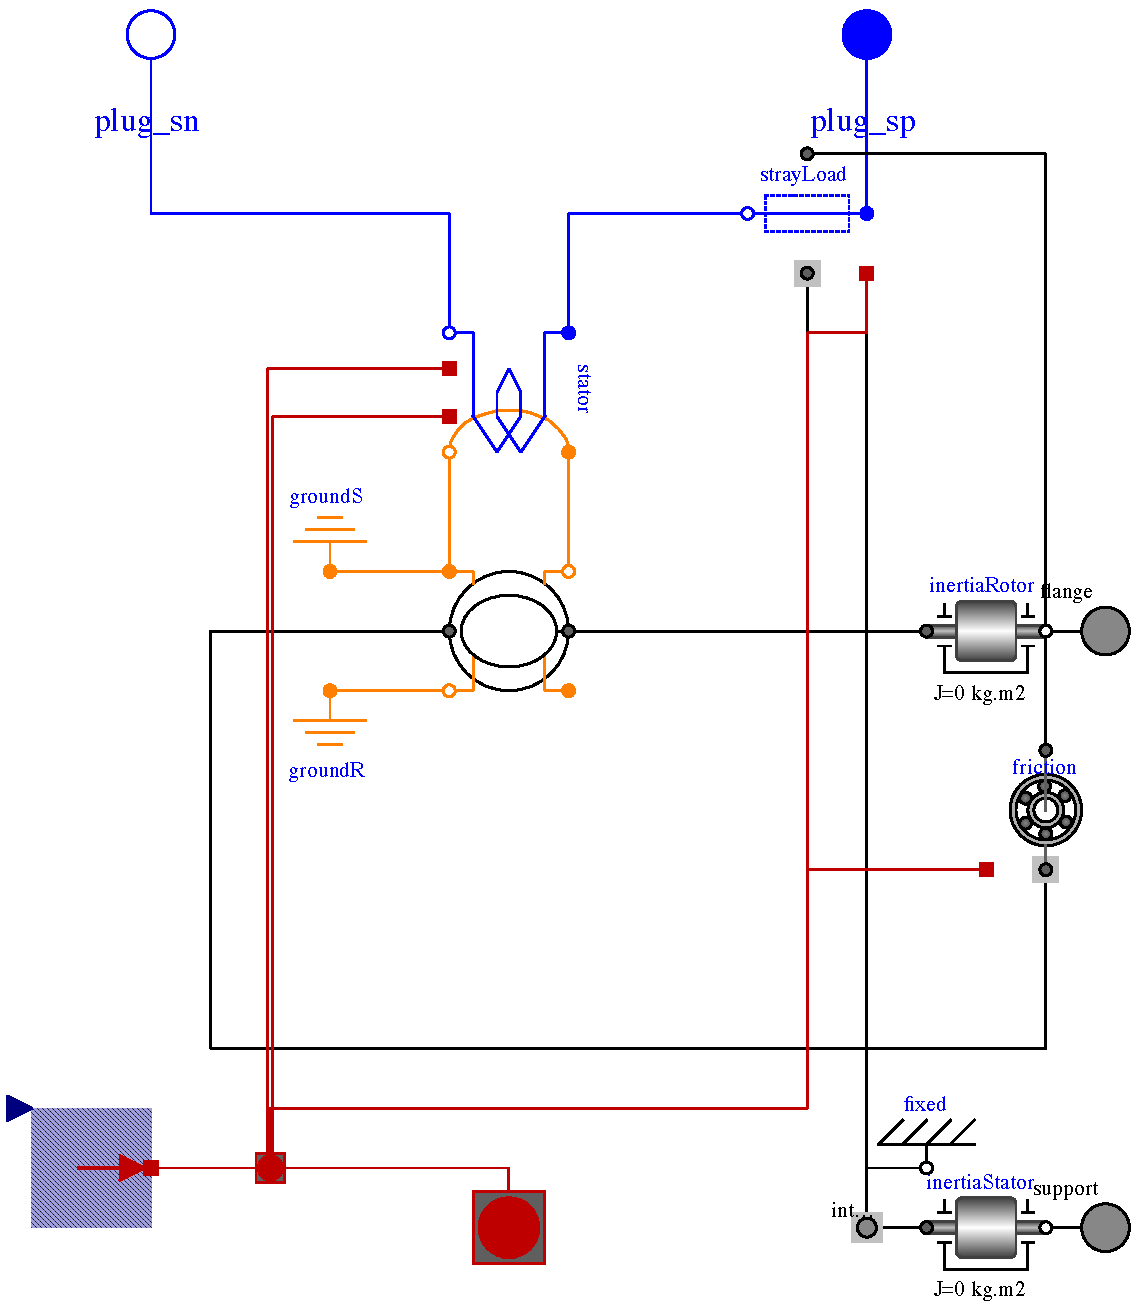
\includegraphics{Bilder/PartialBasicInductionMachine.pdf}
\caption{Partielles Modell der Drehfeldmaschine
\texttt{FundamentalWave.Interfaces.PartialBasicInductionMachine} der MSL
v3.2.3}
\end{figure}

Die Energiewandlung im Stator geschieht über das Windungsmodell
\texttt{FundamentalWave.BasicMachines.Components.SymmetricMultiPhaseWinding},
welches neben der elektro-magnetischen Kopplung auch ohmsche Verluste
sowie Streu- und Wirbelstromverluste des Magnetfelds
berücksichtigt\footnote{Das Modell berücksichtigt bei ungeradzahligen
  mehrphasigen Systemen außerdem noch die Nullinduktivität. Das wird
  jedoch nur benötigt, wenn die Windung unsymmetrisch belastet wird
  (\cite[S. 193]{kralModelicaObjektorientierteModellbildung2019}), was
  in der hier betrachteten Anwendung nicht auftritt.} (siehe XXX).

\begin{figure}
\centering
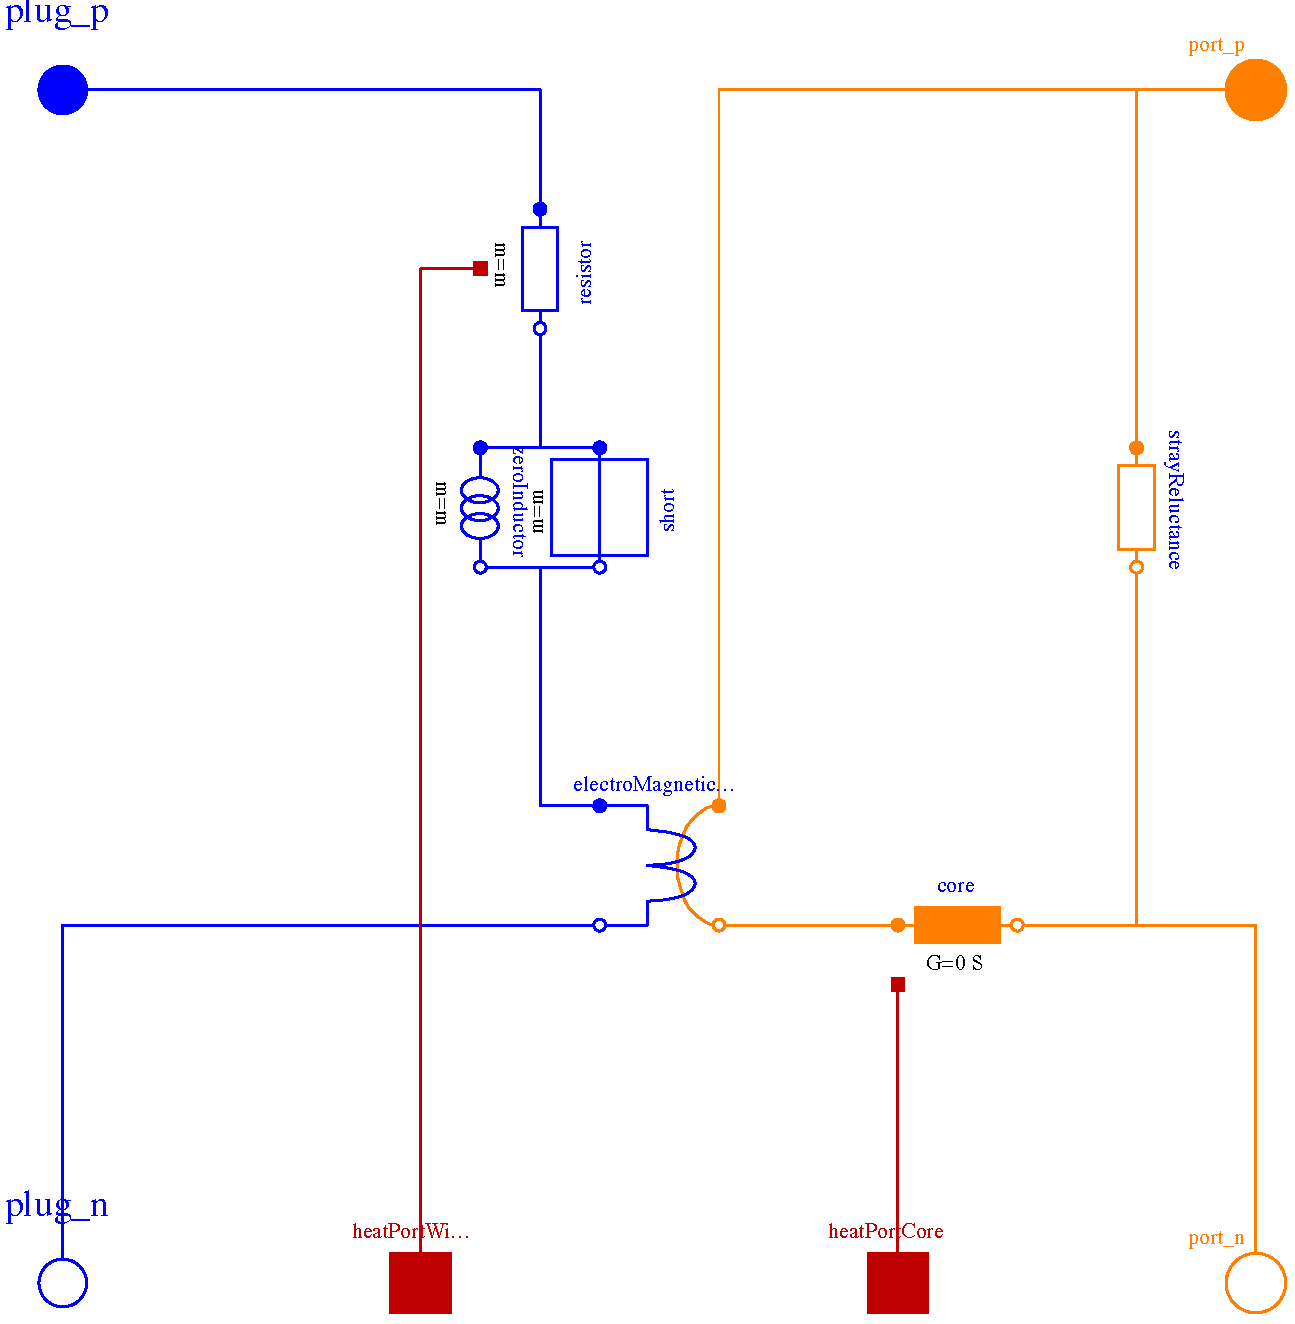
\includegraphics{SymmetricMultiPhaseWinding.pdf}
\caption{Windungsmodell\texttt{FundamentalWave.BasicMachines.Components.SymmetriMultiPhaseWinding}
der MSL v3.2.3}
\end{figure}

Über das Luftspaltmodell
(\texttt{FundamentalWave.BasicMachines.Components.RotorSaliencyAirGap})
wird der Abfall der magnetischen Spannung über dem magnetischen
Widerstand des Luftspalts sowie das auf den Rotor wirkende Drehmoment
modelliert. Um die magnetischen Größen des Stators und des Rotors in
Beziehung zueinander zu setzen ist eine Koordiantentransformation der
Statorgrößen in das körperfeste Bezugssystem des Rotors implementiert
(\emph{d,q-System}).

\hypertarget{modell}{%
\subsubsection{Modell}\label{modell}}

XXX zeigt das vollständige Modell der Asynchronmaschine mit
Kurzschlussläufer
(\texttt{FundamentalWave.BasicMachines.AsynchronousInductionMachines.AIM\_SquirrelCage}).
Es ergibt sich aus dem partiellen Modell durch Hinzufügen des
kurzgeschlossenen Käfigmodells
(\texttt{FundamentalWave.BasicMachines.Components.SymmetricMultiPhaseCageWinding}),
welches XXX zeigt.

Da die Anzahl \(N_R\) der Rotorstäbe eines Käfigs häufig viel größer ist
als die Anzahl \(m\) der Phasen des Systems, ist es numerisch einfacher
für den Käfig eine \(m\)-phasige kurzgeschlossene Windung als
Ersatzmodell zu verwenden, welche die gleiche effektive Windungszahl wie
die Statorwicklung aufweist.
(\cite[S. 194]{kralModelicaObjektorientierteModellbildung2019})

\begin{figure}
\centering
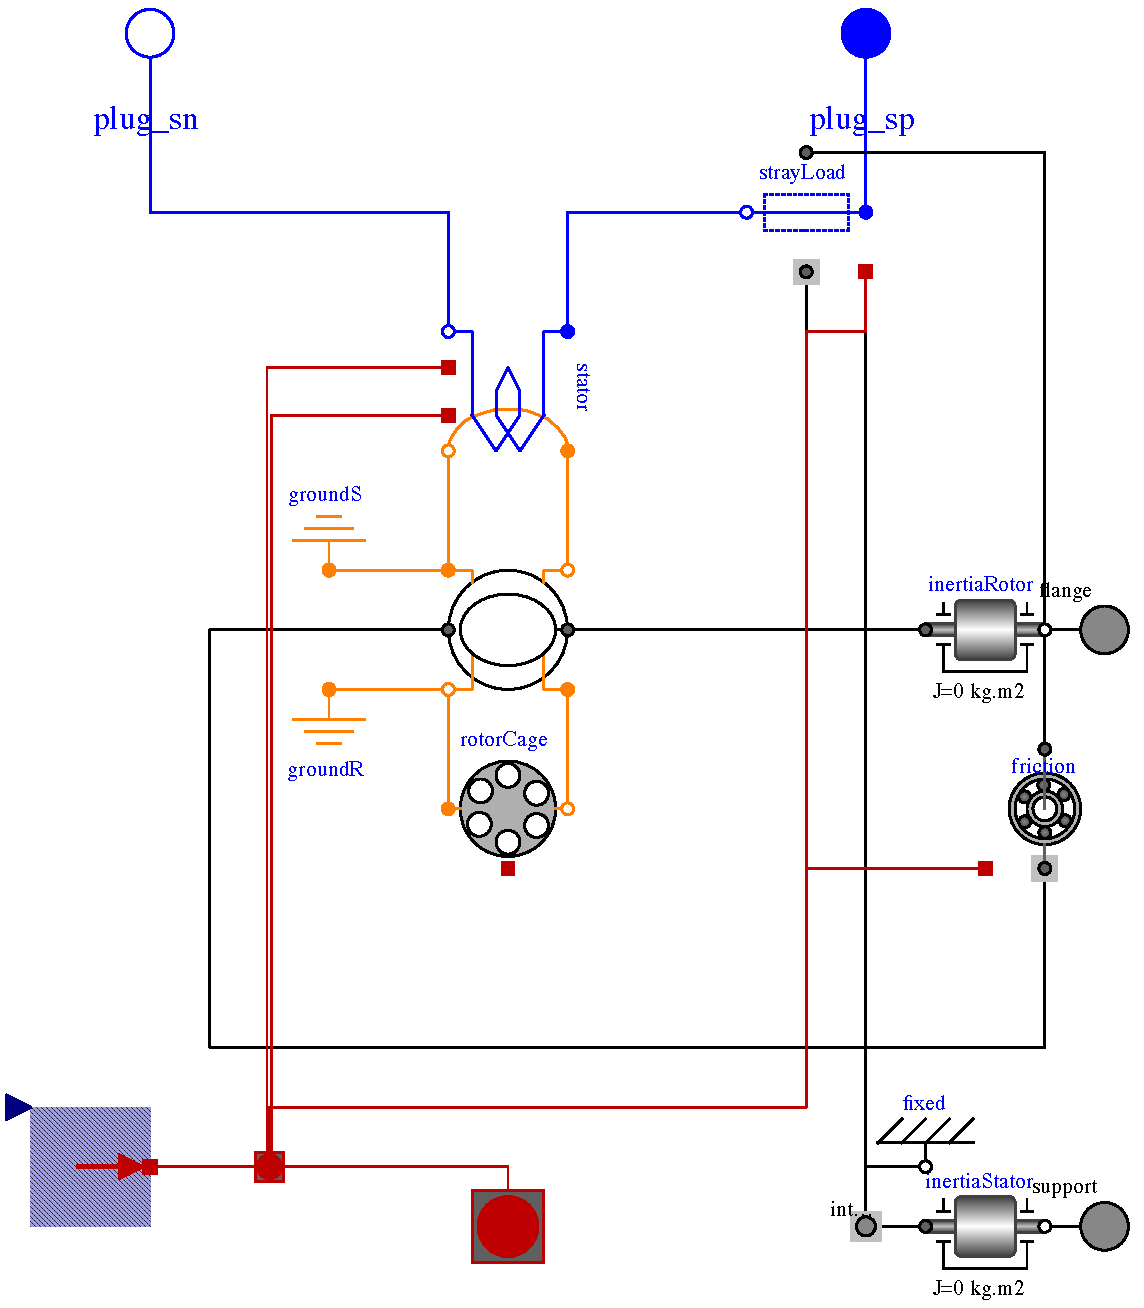
\includegraphics{AIM_SquirrelCage.pdf}
\caption{Vollständiges Modell der Asynchronmaschine mit
Kurzschlussläufer
(\texttt{FundamentalWave.BasicMachines.AsynchronousInductionMachines.AIM\_SquirrelCage})
der MSL v3.2.3}
\end{figure}

\begin{figure}
\centering
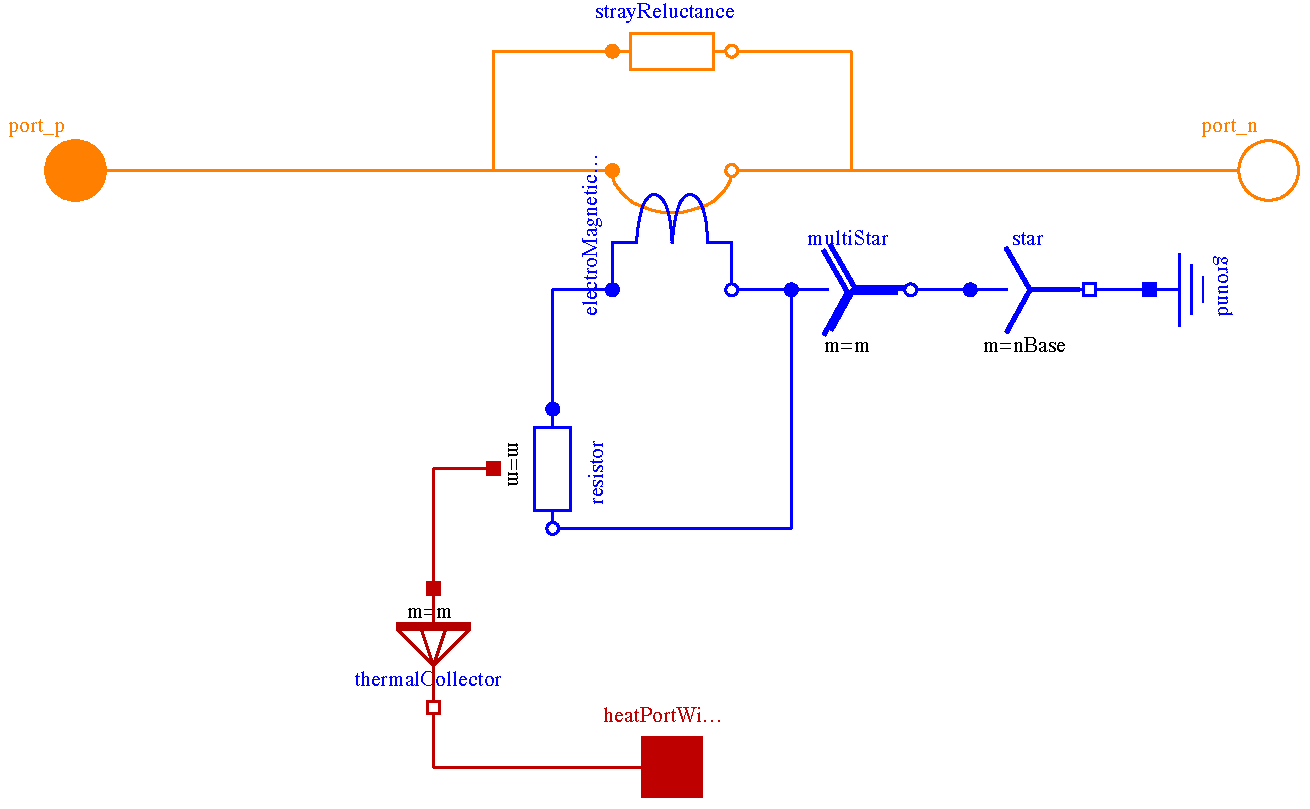
\includegraphics{SymmetricMultiPhaseCageWinding.pdf}
\caption{M-phasiges Käfig-Ersatzmodell
(\texttt{FundamentalWave.Components.SymmetricMultiPhaseCageWinding}) der
MSL v3.2.3}
\end{figure}

\hypertarget{parametrierung}{%
\subsubsection{Parametrierung}\label{parametrierung}}

Zur Parametrierung der Maschine müssen drei Arten von Größen angegeben
werden: elektrische, mechanische und thermische Größen. Da bei
Adaptieren des Frequenzumformer-Modells auf andere Maschinengrößen
vorrangig die elektrischen und mechanischen Größen angepasst werden
müssen, werden diese Werte in einem eigenen Recod-Modell
(\texttt{Frequenzumformer.Maschinenparameter.AIM\_SquirrelCageData},
siehe Listing XXX) zusammengefasst. Das ermöglicht auch die Umrechnung
der im Datenblatt der Maschine angegebenen Reaktanzen in die für die
Simulation benötigten Induktivitäten.

Die thermischen Größen (Betriebspunkts- und Referenztemperaturen von
Stator und Rotor, Temperaturabhängigkeit der Widerstände) werden auf
\(\unit[20]{°C}\) Umgebungstemperatur eingestellt, wobei die
Temperaturabhängigkeit der Widerstände vernachlässigt werden soll.

Wie schon oben erwähnt, verwendet das Modell der Asynchronmaschine nach
außen hin zur Parametrierung der Wicklungen Stator- und
Rotorinduktivitäten, sowie die effektive Statorwindungszahl. Die
Induktivitäten sind die auch im T-Ersatzschaltbild der Maschine (vgl.
XXX) angegeben Größen: Hauptfeldinduktivität (\(L_m\)),
Stator-Streuinduktivität (\(L_{s\sigma}\)) und Rotor-Streuinduktivität
(\(L_{r\sigma}\)). Im Datenblatt der Maschine sind die Reaktanzen
\(X_0, X_1, X_2\) angegeben. Die zugehörigen Induktivitäten ergeben sich
mit der Netzfrequenz \(f_{Netz}=\unit[50]{\mathrm{Hz}}\) nach
\begin{align}
L_m &= \frac{X_0}{2\pi f_{Netz}} \\
L_{s,\sigma} &= \frac{X_1}{2\pi f_{Netz}} \\
L_{r,\sigma} &= \frac{X_2}{2\pi f_{Netz}}.
\end{align}
Für die effektive Windungszahl (\texttt{effectiveStatorTurns}) gibt
\cite[S. 217]{kralModelicaObjektorientierteModellbildung2019}
\begin{equation}
N_{\mathrm{eff. s}} = \hat{N}\cdot\xi_{\mathrm{c}}\cdot\xi_{\mathrm{z}},
\end{equation}
an, mit der \emph{Statorwindungszahl} \(\hat{N}\), dem
\emph{Sehnungsfaktor} \(\xi _{\mathrm{c}}\) und dem \emph{Zonenfaktor}
\(\xi _{\mathrm{z}}\). Ebenda angegeben sind die Ausdrücke XXX für die
beiden Faktoren \(\xi _{\mathrm{c}}\) und \(\xi_{\mathrm{z}}\)
(\cite[S. 165, S. 217]{kralModelicaObjektorientierteModellbildung2019}).
\begin{align}
\xi _{\mathrm{c}} &= \sin(\frac{\Delta\gamma _{\mathrm{c}}}{2}) \\
\xi _{\mathrm{z}} &= \frac{\sin(\frac{\pi}{6})}{q\sin(\frac{\pi}{6q})}
\end{align}
Die \emph{Spulenweite} \(\Delta\gamma _{\mathrm{c}}\) ist gemäß
\begin{equation}
\Delta\gamma _{\mathrm{c}} = 2\pi\cdot\frac{y _{\mathrm{Q}}}{S'}
\end{equation}
das Verhältnis des \emph{Nutschritts} (\(y_Q\)) zur Anzahl der
\emph{Nuten je Polpaar} (\(S'=\sfrac{Q}{2p}\)) multipliziert mit
\(2\pi\)
(\cite[S. 168, S. 161]{kralModelicaObjektorientierteModellbildung2019}),
vgl. \cite[S. 76, S. 119]{binderElektrischeMaschinenUnd2012}). Ebenso
ist die \emph{Lochzahl} (\(q\)) zur Berechnung des Zonenfaktors das
Verhältnis der Anzahl der Nuten zur Anzahl der Stränge und Pole (vgl.
\cite[S. 151]{kralModelicaObjektorientierteModellbildung2019})
\begin{equation}
q = \frac{Q}{2pm}.
\end{equation}
Damit ist die Statorwindung der Asynchronmaschine vollständig
parametriert. Die Wicklungsdaten und die daraus nach XXX berechneten
Werte listet XXX auf. Alle weiteren Größen zur Beschreibung der
Asynchromaschine können direkt aus dem Datenblatt entnommen und sind
ebenfalls in XXX angegeben.

Dabei ist für das Trägheitsmoment \(J_{\mathrm{r}}=0\) eingetragen, da
aus der Auslegung des Frequenzumformer nur ein kombiniertes
Trägheitsmoment der Welle mit den Rotoren aller drei Maschinen und dem
Lüfter bekannt ist. Da die die Modellierung der Welle starr (d.h. ohne
Berücksichtigung der Elastizität oder der inneren Dämpfung der Welle)
geschieht, kann dieses kombinierte Trägheitsmoment im Trägheitsmoment
des Lüftermodells zusammengefasst werden.

\hypertarget{synchrongenerator-mit-duxe4mpferkuxe4fig}{%
\subsection{Synchrongenerator mit
Dämpferkäfig}\label{synchrongenerator-mit-duxe4mpferkuxe4fig}}

Das Modell des Synchrongenerators basiert wie auch das der
Asynchronmaschine auf dem oben schon dargestellten partiellen
Drehfeldmaschinenmodell. Es fügt dem partiellen Modell ein einphasiges
elektro-magnetisches Kopplungsmodell und ein Bürstenmodell für die
elektrische Erregung hinzu und bietet einen optionalen Dämpferkäfig,
ähnlich zu dem Kurzschlussläufer der Asynchronmaschine.

\hypertarget{modell-1}{%
\subsubsection{Modell}\label{modell-1}}

XXX zeigt das vollständige Modell des elektrisch erregten
Synchrongenerators mit Dämpferkäfig. Die Verwendung des Dämpferkäfigs
wird über den Parameter \texttt{useDamperCage} eingestellt. Wird dieser
Parameter auf \texttt{false} gesetzt, wird das Modell mit dem
Verbindungsmodell \texttt{short} anstelle des Dämpferkäfigs
initialisiert. 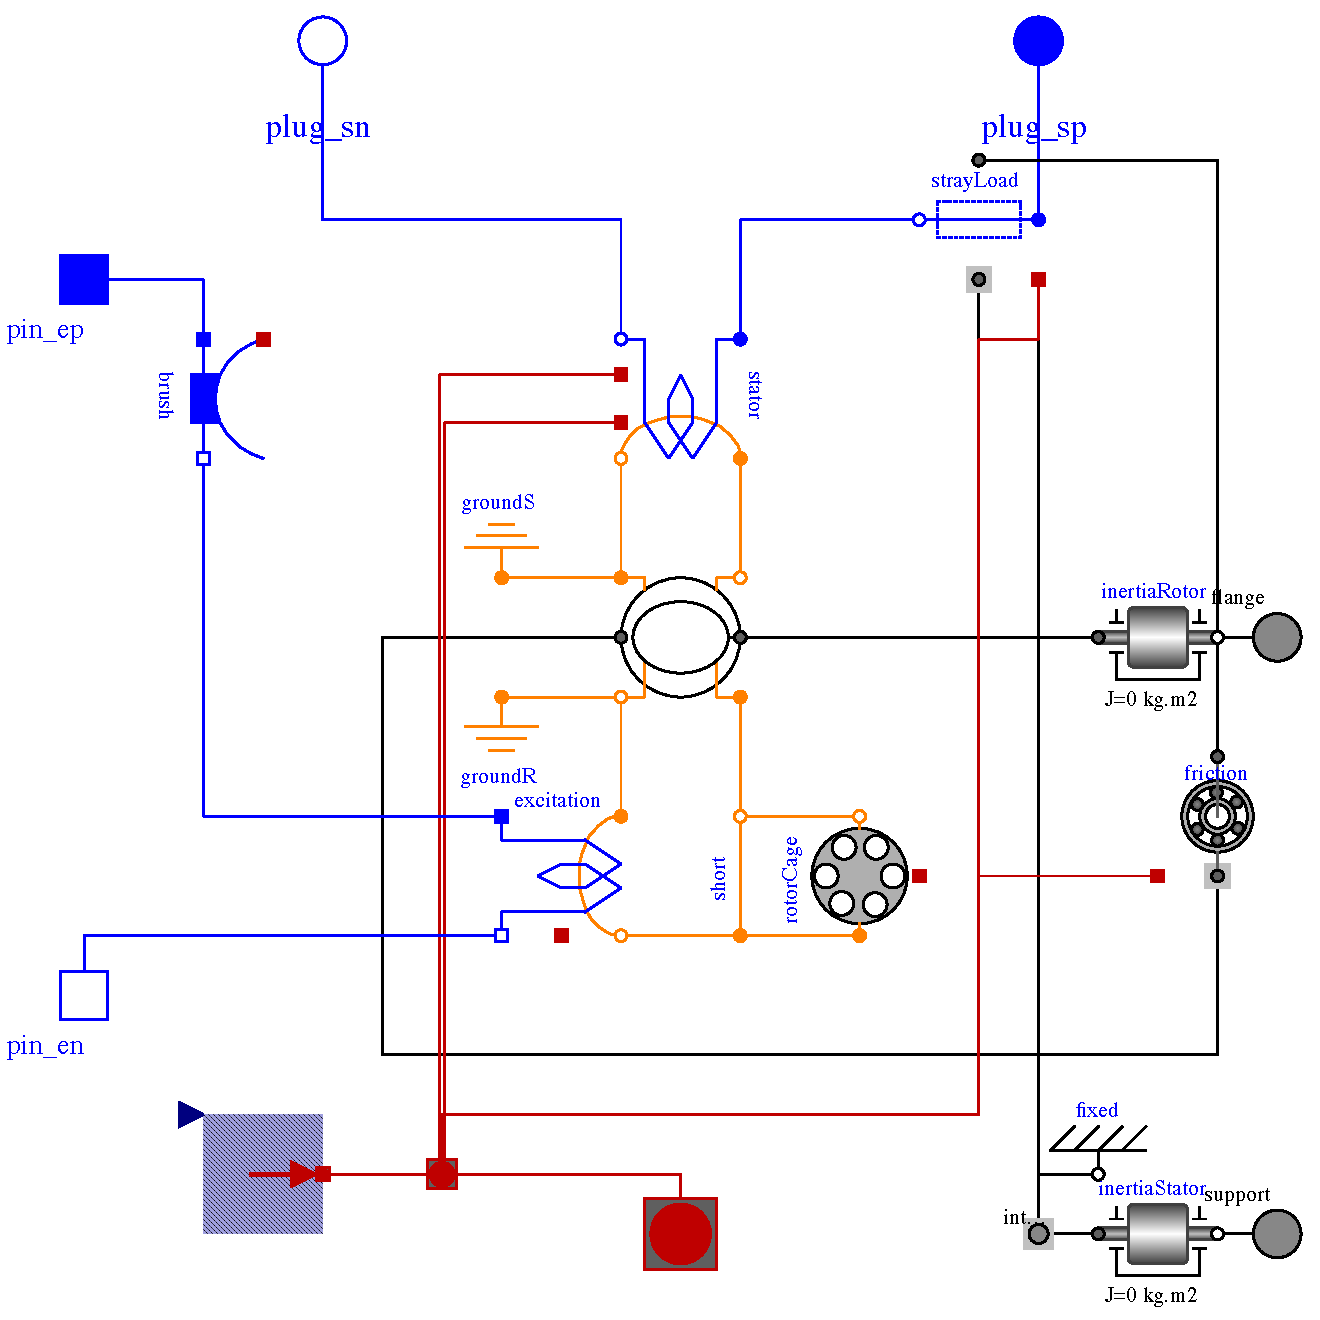
\includegraphics{SM_ElectricalExcited.pdf}

Wie das mehrphasige Windungsmodell des Stators (siehe XXX)
berücksichtigt auch das einphasige Modell neben der elektromagnetischen
Kopplung ohmsche Verluste und den magnetischen Streufluss (siehe XXX).
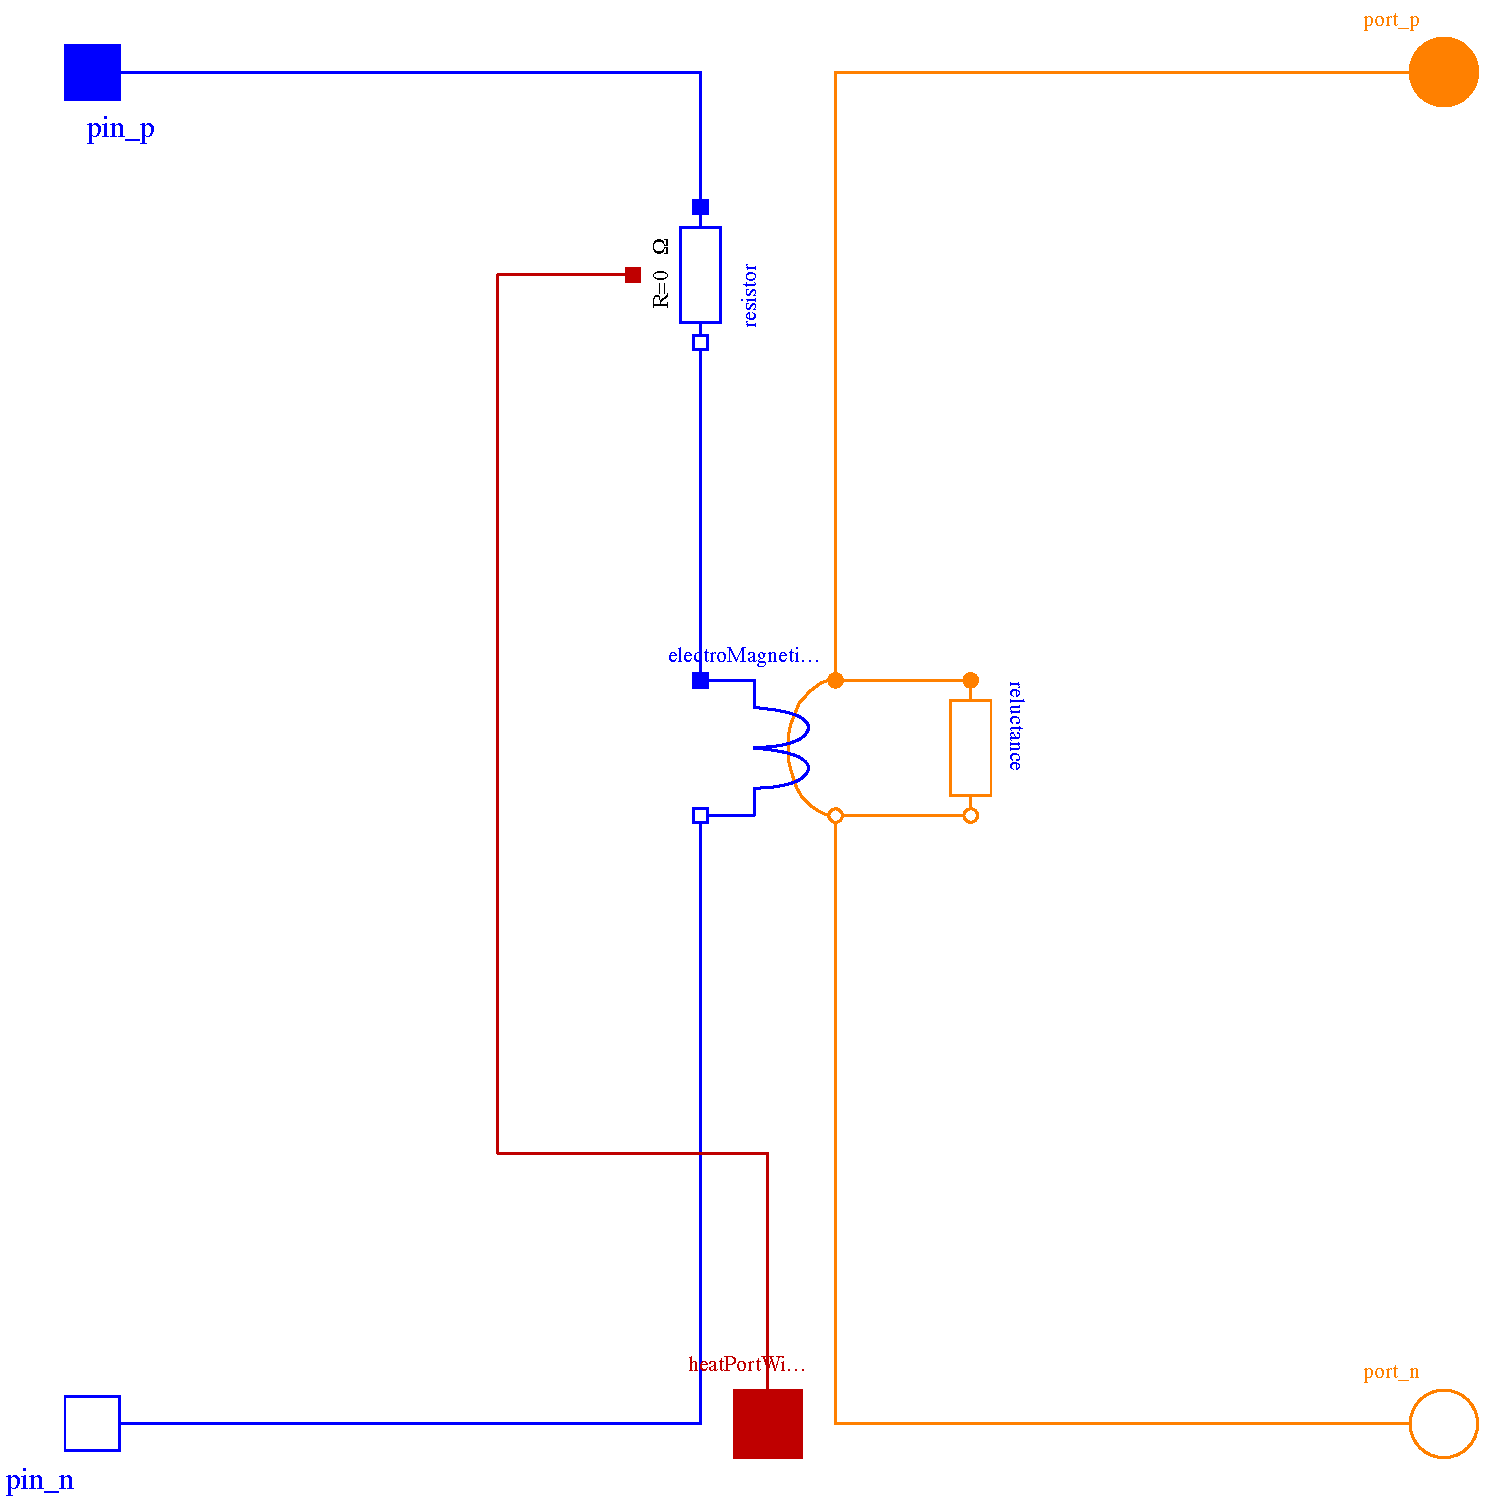
\includegraphics{SinglePhaseWinding.pdf}

Da der Synchrongenerator über die Erregermaschine erregt wird, findet
keine Stromübertragung über Kohlebürsten statt und das Modell der
Kohlebürsten soll hier nicht beschrieben werden. Weiterhin beträgt der
Spannungsabfall über den Kohlebürsten in der Voreinstellung Null Volt.
Daher brauchen für die Kohlebürsten keine Parameter angegeben zu werden,
um einen Einfluss auszuschließen.

Das Modell des Dämpferkäfigs (siehe XXX) weist die gleiche Struktur auf
wie der oben beschriebene Kurzschlussläufer. Im Unterschied zu diesem
berücksichtigt das Dämpferkäfigmodell hingegen eine Achsigkeit (d- und
q-Achsen des körperfesten Koordinatensystems) der Widerstände und
Induktivitäten aufgrund der Pollücken des Dämpferkäfigs
(\cite[S. 194]{kralModelicaObjektorientierteModellbildung2019}).
Dementsprechend ist das Modell zweiphasig
ausgeführt.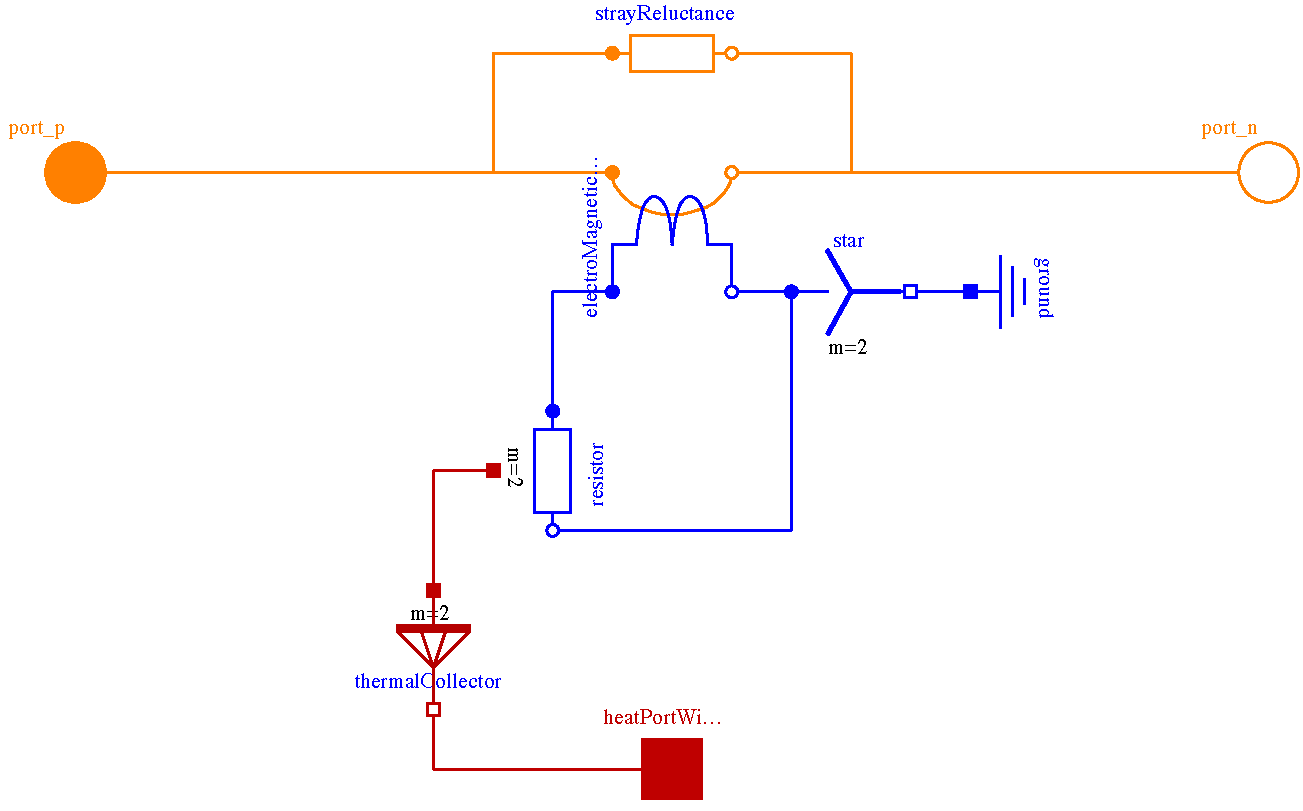
\includegraphics{SaliencyCageWinding.pdf}

\hypertarget{parametrierung-1}{%
\subsubsection{Parametrierung}\label{parametrierung-1}}

Alle Parameter des Synchrongenerators werden in Parameterrecord
\texttt{Machines.Utilities.ParameterRecords.SM\_ElectricalExcitedData}
der MSL v3.2.3 erfasst. Die mechanischen und thermischen Parameter des
Synchrongenerators sind dieselben wie die der Asynchronmaschine: Die
Temperaturen betragen \(\unit[20]{°C}\) Umgebungstemperatur bei
Vernachlässigung der Temperaturabhängigkeit der Widerstände und das
Trägheitsmoment wird ebenfalls in dem kombinierten Trägheitsmoment des
Lüfters erfasst.

Die zur Parametrierung des Synchrongenerators verwendeten elektrischen
Größen sind die im Erstzschaltbild XXX angegebenen Widerstände und
Induktivitäten. Aus der Auslegung der Maschine hingegen sind die in
Tabelle XXX aufgelisteten Größen bekannt. Die zur Umrechnung benötigten
Zusammenhänge sollen im Folgenden angegeben werden.\footnote{Die hier
  angegebenen Zusammenhänge sind zum größten Teil auch in dem
  Parameterrecord \texttt{Machines.Utilities.SynchronousMachineData}
  implementiert, erforden jedoch die Kenntnis der Ankerzeitkonstante
  \(T_{\mathrm{a}}\) zur Berechnung des Statorwiderstands
  \(R_{\mathrm{s}}\). Da jedoch \(R_{\mathrm{s}}\) (im Gegensatz zu
  \(T_{\mathrm{a}}\)) aus der Auslegung bekannt ist, erfolgt hier diese
  angepasste Umformung der Kenngrößen.}

Nach \cite[S. 264]{kralModelicaObjektorientierteModellbildung2019}
können die bezogenen Hauptfeldreaktanzen \(x_{\mathrm{md}}\) und
\(x_{\mathrm{mq}}\) mit
\begin{align}
x_{\mathrm{md}} &= x_{\mathrm{d}} - x_{\mathrm{s}} \\
x_{\mathrm{mq}} &= x_{\mathrm{q}} - x_{\mathrm{s}}
\end{align}
aus den bezogenen Reaktanzen \(x_{\mathrm{d}}\) und \(x_{\mathrm{q}}\)
sowie der Streureaktanz \(x_{\mathrm{s}}\) bestimmt werden.\footnote{An
  dieser Stelle verwendet
  \cite[]{kralModelicaObjektorientierteModellbildung2019} anstelle von
  \(x_{\mathrm{s}}\) die Nullreaktanz \(x_{\mathrm{0}}\), die in etwa
  mit der Streureaktanz übereinstimmt. Da hier aber die Streureaktanz
  aus der Auslegung bekannt ist, soll \(x_{\mathrm{s}}\) direkt
  verwendet werden.} Weiterhin wird dort die Reaktanz der
Erregerwicklung gemäß
\begin{equation}
x_{\mathrm{e}} = \frac{x_{\mathrm{md}}^2}{x_{\mathrm{d}}-x_{\mathrm{d}}'}
\end{equation}
angegeben. Ebenso seien die Zusammenhänge für die bezogenen
Rotorreaktanzen \(x_{\mathrm{rd}}\) und \(x_{\mathrm{rq}}\)
\begin{align}
x_{\mathrm{rd}} &= \frac{x_{\mathrm{md}}^2}{x_{\mathrm{d}}’ - x_{\mathrm{d}}''}\cdot \left( 1-\frac{x_{\mathrm{md}}}{x_{\mathrm{d}}}\right)^2 + \frac{x_{\mathrm{md}}^2}{x_{\mathrm{e}}}\\
\intertext{und}
x_{\mathrm{rq}} &= \frac{x_{\mathrm{mq}}^2}{x_{\mathrm{q}} - x_{\mathrm{q}}''}.
\end{align}
Für die bezogenen Rotorwiderstände\footnote{An dieser Stelle liegt in
  der vorliegenden Ausgabe von
  \cite[]{kralModelicaObjektorientierteModellbildung2019} ein
  Druckfehler vor (vgl. mit dem Modelica-Code Listing
  \cite[S. 266]{kralModelicaObjektorientierteModellbildung2019})} wird
ebenda
\begin{align}
r_{\mathrm{rd}} &= \frac{x_{\mathrm{rd}} - \frac{x_{\mathrm{md}}^2}{x_{\mathrm{e}}}}{\omega_{\mathrm{sN}}\cdot T_{\mathrm{d0}}''}, \\
r_{\mathrm{rq}} &= \frac{x_{\mathrm{rq}}}{T_{\mathrm{q0}}''}
\end{align}
angegeben und für den bezogenen Widerstand der Erregerwicklung
 \begin{equation}
r_{\mathrm{e}} = \frac{x_{\mathrm{e}}}{\omega_{\mathrm{sN}}\cdot T_{\mathrm{d0}}''}.
\end{equation}
Die beiden Subtransienten Leerlaufzeitkonstanten \(T_{\mathrm{d0}}''\)
und \(T_{\mathrm{q0}}''\) sind nach
\cite[S. 222ff.]{bonfertBetriebsverhaltenSynchronmaschine1962} über den
Zusammenhang
\begin{align}
T_{\mathrm{d0}}'' &= \frac{x_{\mathrm{d}}'}{x_{\mathrm{d}}''}T_{\mathrm{d}}'' \\
T_{\mathrm{q0}}'' &= \frac{x_{\mathrm{q}}}{x_{\mathrm{q}}''}T_{\mathrm{q}}
\end{align}
aus den Kurzschlusszeitkonstanten \(T_{\mathrm{d}}''\) und
\(T_{\mathrm{q}}''\) berechenbar.

Damit ergeben sich die Induktivitäten und Widerstände des
Synchrongenerators mit der Nennkreisfrequenz
\(\omega_{\mathrm{sN}}=2\pi\cdot f_{\mathrm{sN}}\) und der
Bezugsreaktanz \(X_{\mathrm{N}}\) nach Gleichungen XXX (vgl.
\cite[S.265f.]{kralModelicaObjektorientierteModellbildung2019}).
\begin{align}
L_{\mathrm{md}} &= x_{\mathrm{md}}\cdot \frac{X_{\mathrm{N}}}{\omega_{\mathrm{sN}}} \\
L_{\mathrm{mq}} &= x_{\mathrm{mq}}\cdot \frac{X_{\mathrm{N}}}{\omega_{\mathrm{sN}}} \\
L_{\mathrm{r \sigma d}} &= (x_{\mathrm{rq}}-x_{\mathrm{mq}})\cdot \frac{X_{\mathrm{N}}}{\omega_{\mathrm{sN}}} \\
L_{\mathrm{r \sigma q}} &= (x_{\mathrm{rd}}-x_{\mathrm{md}})\cdot \frac{X_{\mathrm{N}}}{\omega_{\mathrm{sN}}} \\
L_{\mathrm{s \sigma}} &= x_{\mathrm{s}}\cdot \frac{X_{\mathrm{N}}}{\omega_{\mathrm{sN}}} \\
R_{\mathrm{rd}} &= r_{\mathrm{rd}}\cdot X_{\mathrm{N}} \\
R_{\mathrm{rq}} &= r_{\mathrm{rq}}\cdot X_{\mathrm{N}} \\
R_{\mathrm{e}} &= \frac{3}{2}\cdot \left(\frac{\sqrt{2}V_{\mathrm{sN}}}{\omega_{\mathrm{sN}}L_{\mathrm{md}}\cdot I_{\mathrm{Err. Leerl.}}}\right)^2\cdot r_{\mathrm{e}}\cdot X_{\mathrm{N}}
\end{align}
Damit ist der Synchrongenerator vollständig parametriert. Die Tabellen
XXX listen eine Übersicht über alle Parameter und Berechnungsgrößen auf.

\hypertarget{erregermaschine}{%
\subsection{Erregermaschine}\label{erregermaschine}}

Die Erregermaschine und der auf dem Polrad der Mschine mitrotierende
Gleichrichter dienen gemäß Abb XXX der berührungslosen Erregung des
Synchrongenerators über den Luftspalt. Wie bei dem Hauptgenerator
handelt es sich auch bei der Erregermaschine um eine Synchronmaschine.
Neben der geringeren Größe (ermöglicht durch die geringere
Übertragungsleistung) unterscheiden sich die beiden Generatoren darin,
dass die Erregermaschine eine Innenpol- und der Hauptgenerator eine
Außenpolmaschine ist. In der Modellierung der Maschinen braucht dieser
Umstand jedoch nicht berücksichtigt zu werden. \textgreater{}
{[}!IMPORTANT{]} Diodenmodell erklären

\hypertarget{modell-2}{%
\subsubsection{Modell}\label{modell-2}}

Abb XXX zeigt das vollständige Modell der in der
\texttt{Frequenzumformer}-Bibliothek implementierten Erregermaschine.
Als Generatormodell wird dasselbe Synchrongeneratormodell der MSL wie
für den Hauptgenerator verwendet. Das \texttt{delta}-Modell zwischen den
beiden Ausgängen dreiphasigen Ausgängen des Generators bewirkt eine
Verkettung der Ströme und Spannungen wie in einer Dreieckschaltung der
Statorstränge.

Die Gleichrichtung der erzeugten dreiphasigen Spannung geschieht mit
einem 6-Puls-Brückengleichrichter (siehe Abb XXX). Am negativen Ausgang
des Brückengleichrichters wird ein \(\unit[0]{V}\) Referenzpotential
verschaltet, ohne das die Gleichungen für den elektrischen Kreis
zwischen Erregermaschine und Synchrongenerator nicht eindeutig lösbar
wären. 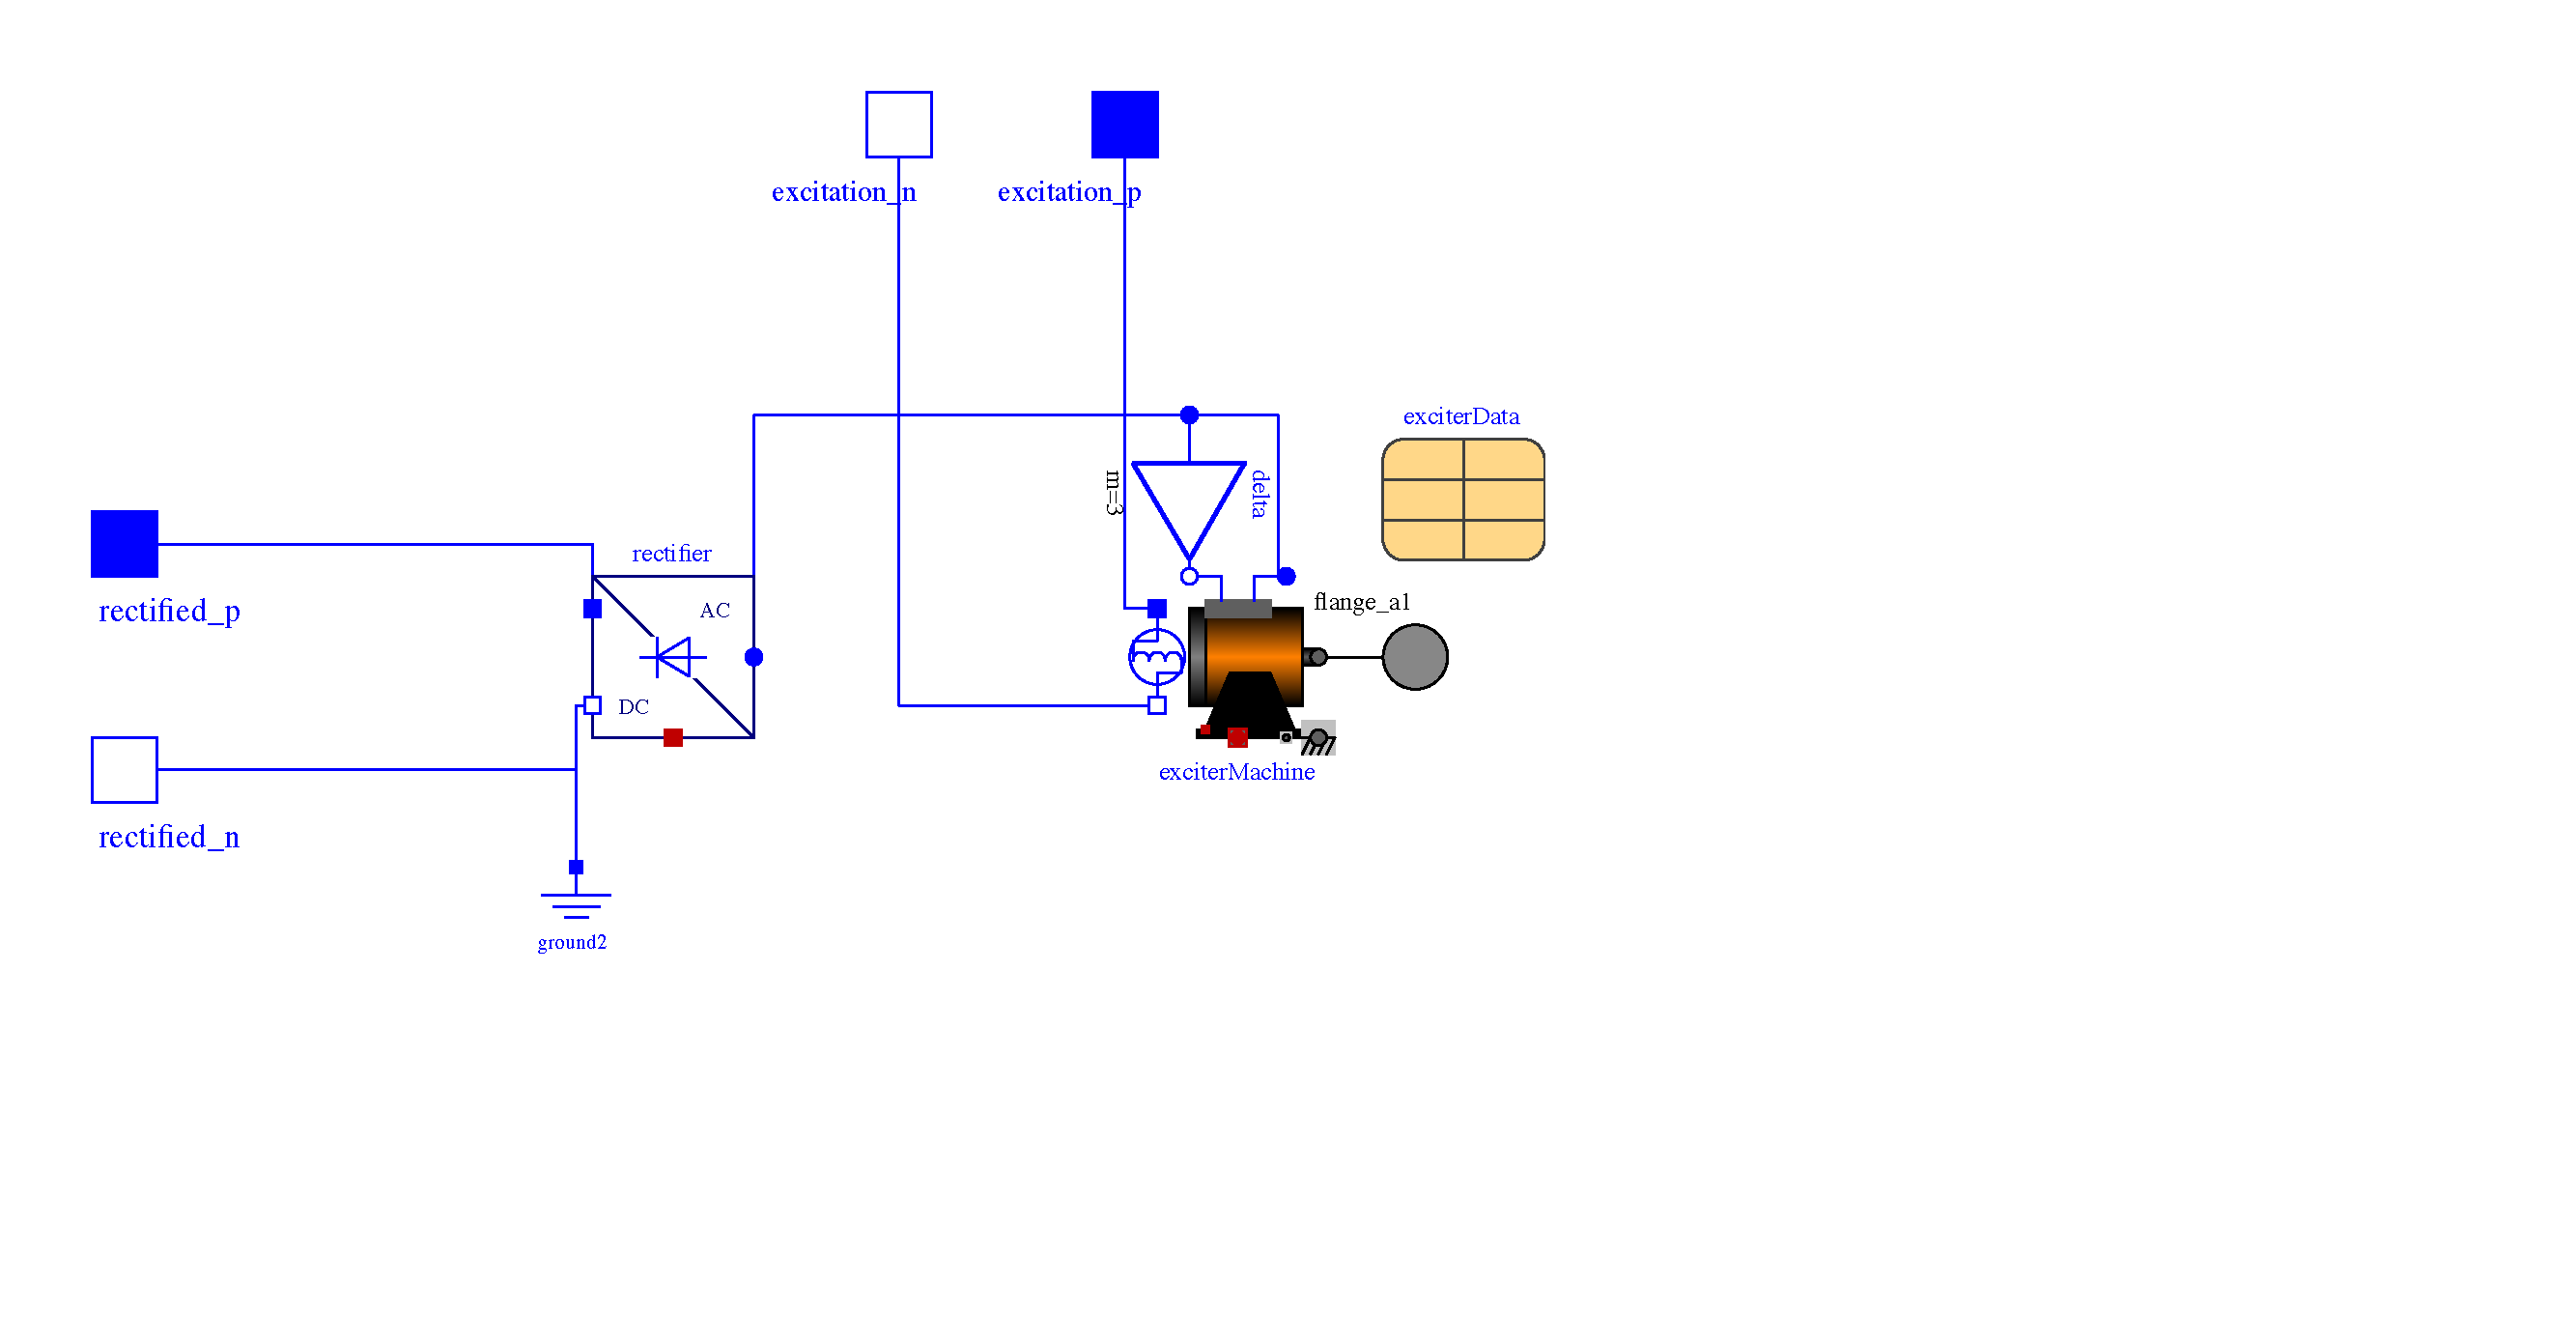
\includegraphics{SM_Erreger.pdf}
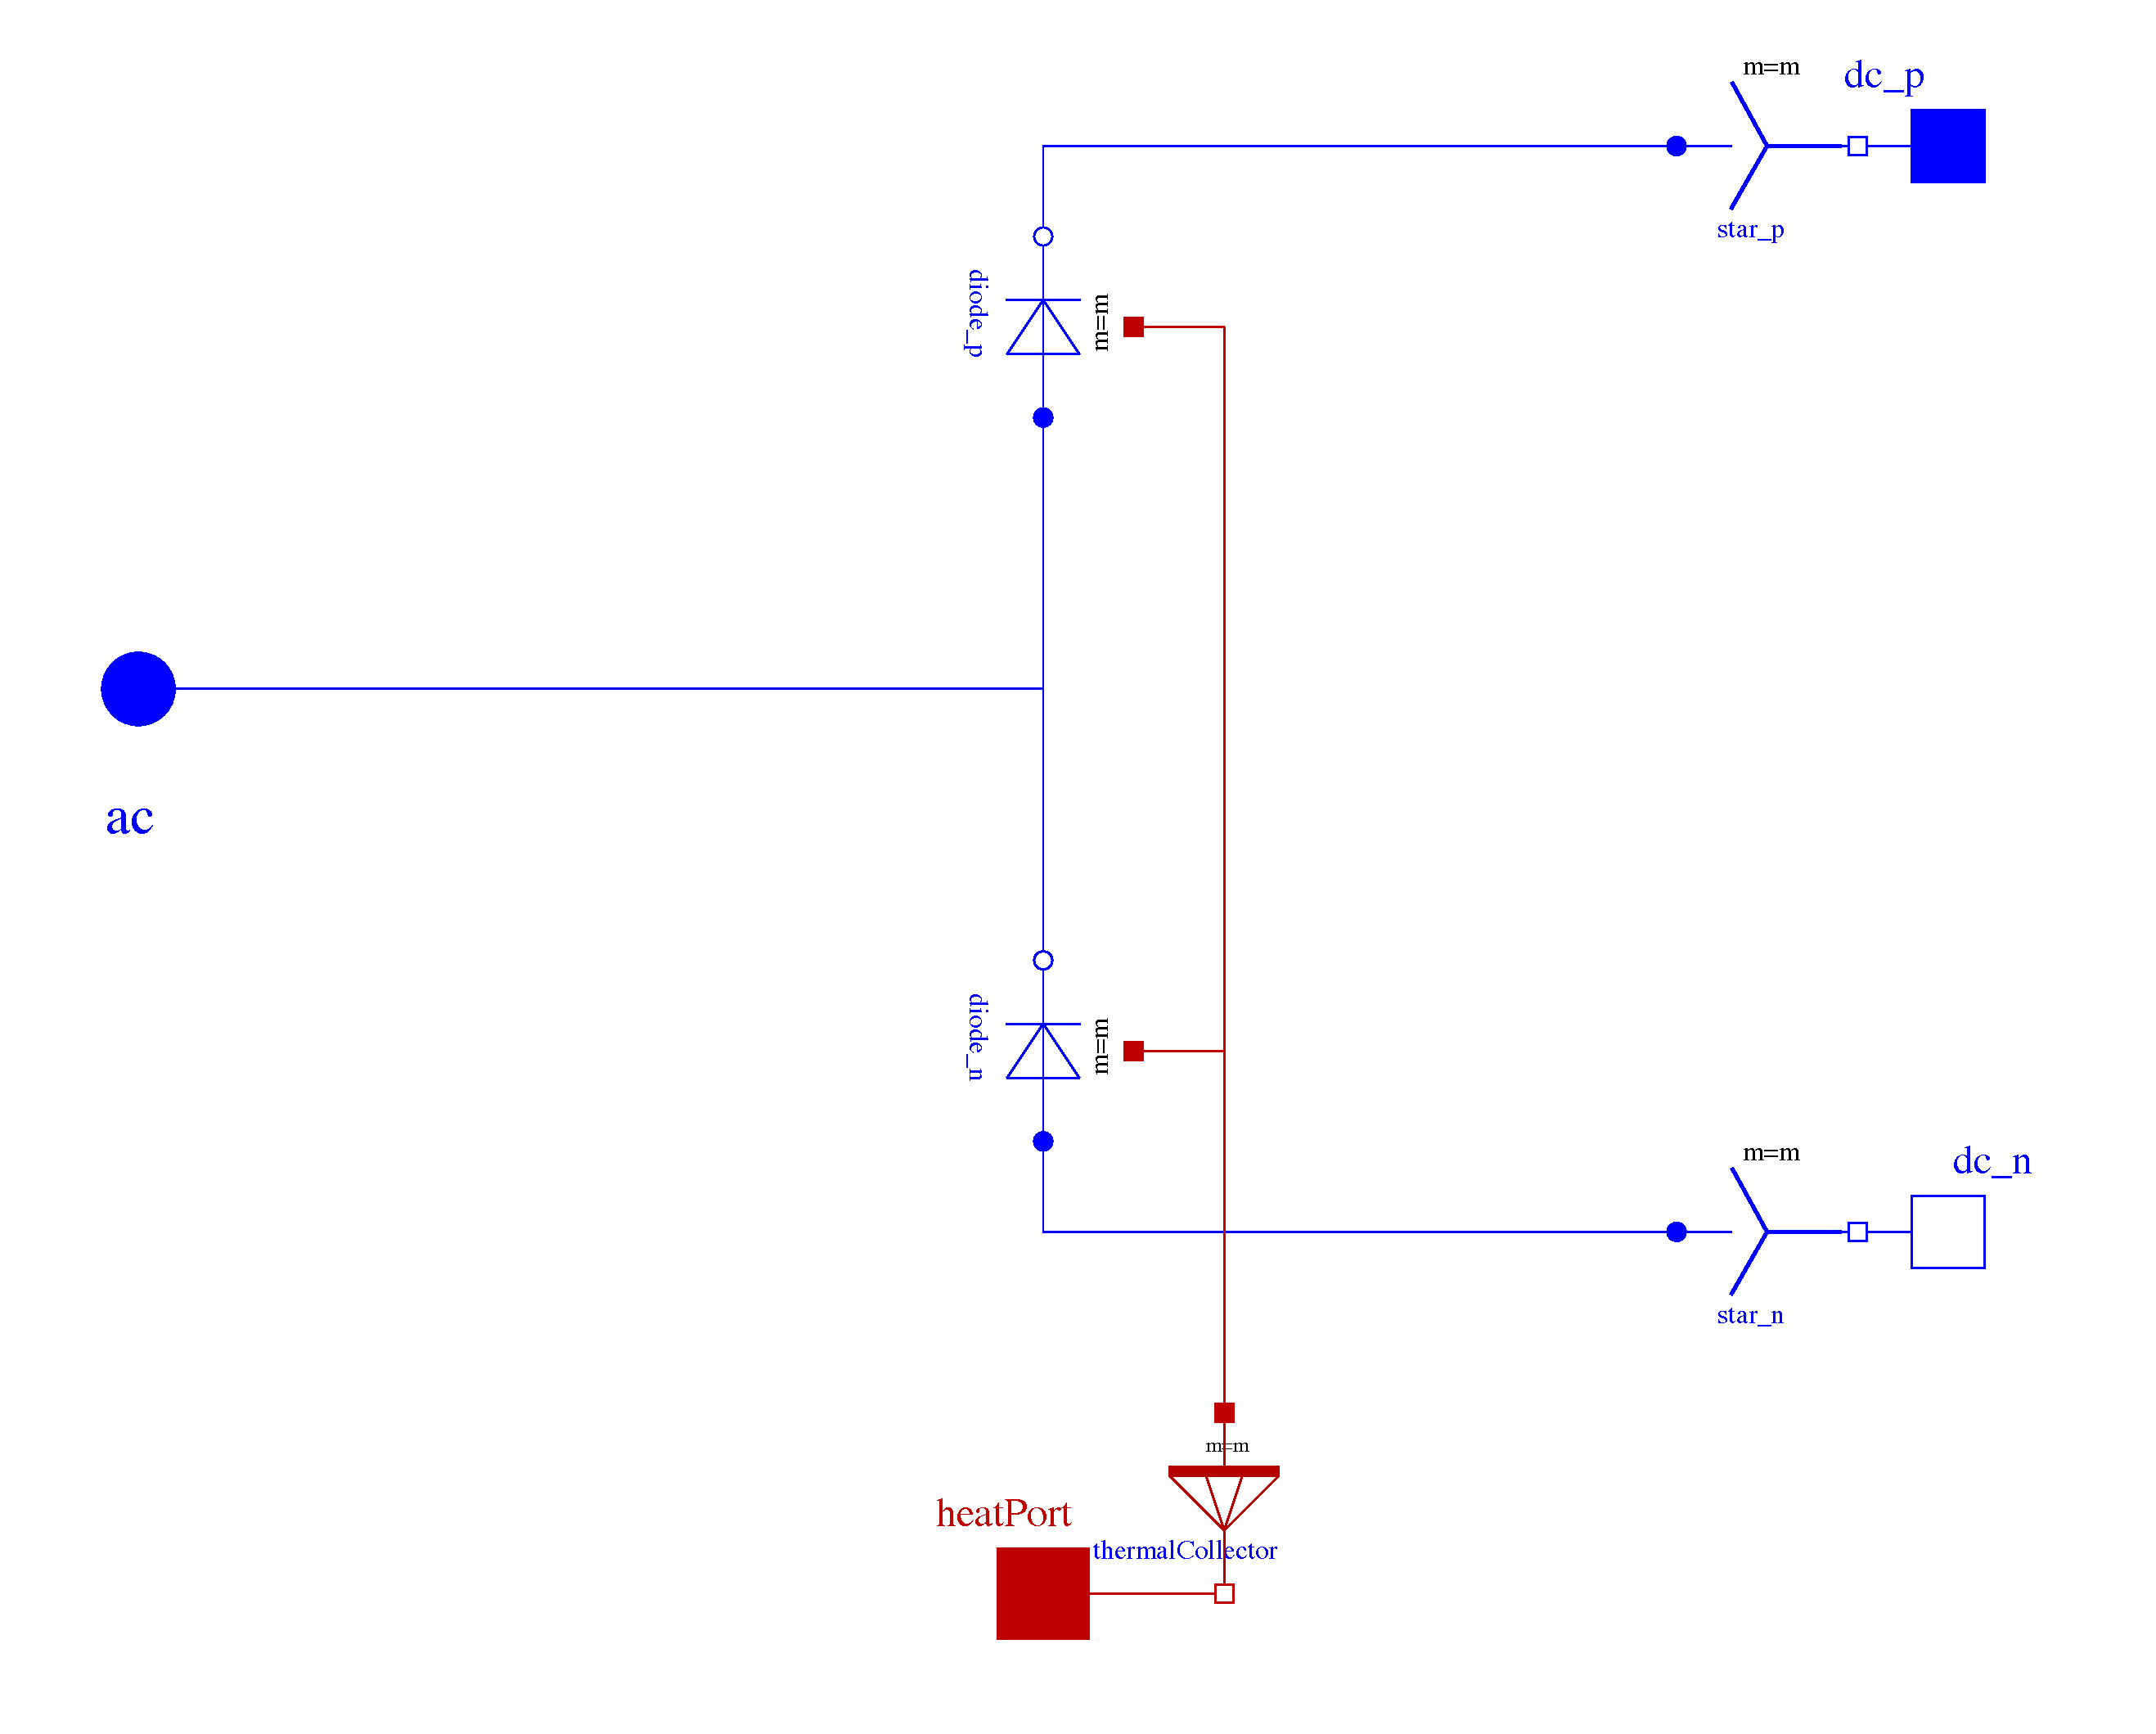
\includegraphics{Bilder/DiodeBridge2mPulse.pdf}

\hypertarget{parametrierung-2}{%
\subsubsection{Parametrierung}\label{parametrierung-2}}

Die Parametrierung des Synchrogenerators der Erregermaschine erfolgt
analog zur Parametrierung des Hauptgenerators oben. Die verwendeten
Größen sind in Tabelle XXX dargestellt.

Für den Brückengleichrichter sind aus der Auslegung keine Werte bekannt.
Daher wird für die Flussspannung \(U_{\mathrm{F}}=\unit[0,7]{V}\)
angenommen. Der Leitwert \(G_{\mathrm{off}}\) im Sperrbetrieb und der
Widerstand \(R_{\mathrm{on}}\) im Durchlassbetrieb einer idealen Diode
betragen Null. Um jedoch numerische Probleme (Teilen durch Null bzw.
Ansteigen der resultierenden Größen gegen Unendlich) zu vermeiden,
werden \(G_{\mathrm{off}}=\unit[0,001]{S}\) bzw.
\(R_{\mathrm{on}}=\unit[0,001]{\Omega}\) festgelegt, die nahe Null, aber
noch groß genug, sind um die genannten Probleme zu vermeiden.

\hypertarget{spannungsregler}{%
\subsection{Spannungsregler}\label{spannungsregler}}

\hypertarget{modell-3}{%
\subsubsection{Modell}\label{modell-3}}

\begin{figure}
\centering
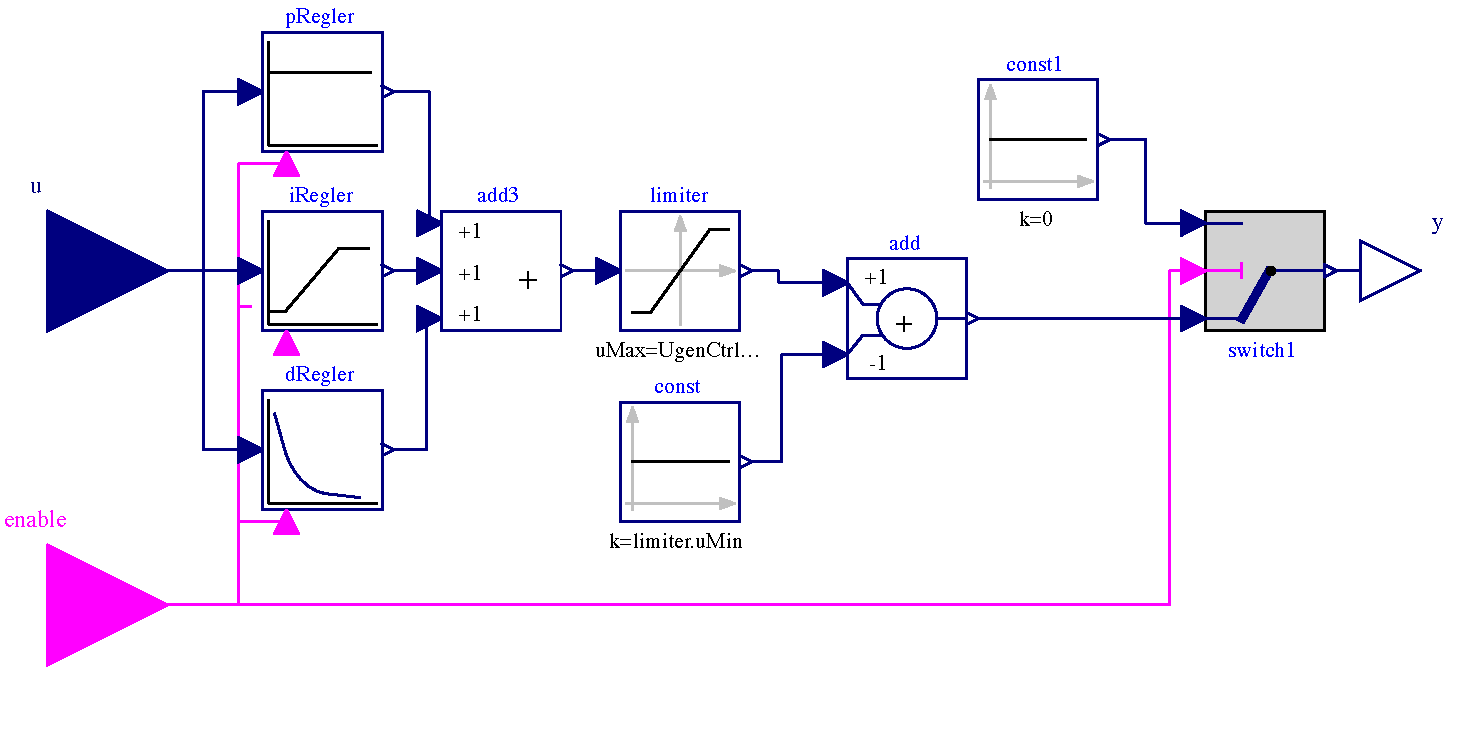
\includegraphics{Bilder/Spannungsregler.pdf}
\caption{Vollständiges Modell des Spannungsreglers
(\texttt{Frequenzumformer.Regler.Spannungsregler})}
\end{figure}

\begin{figure}
\centering
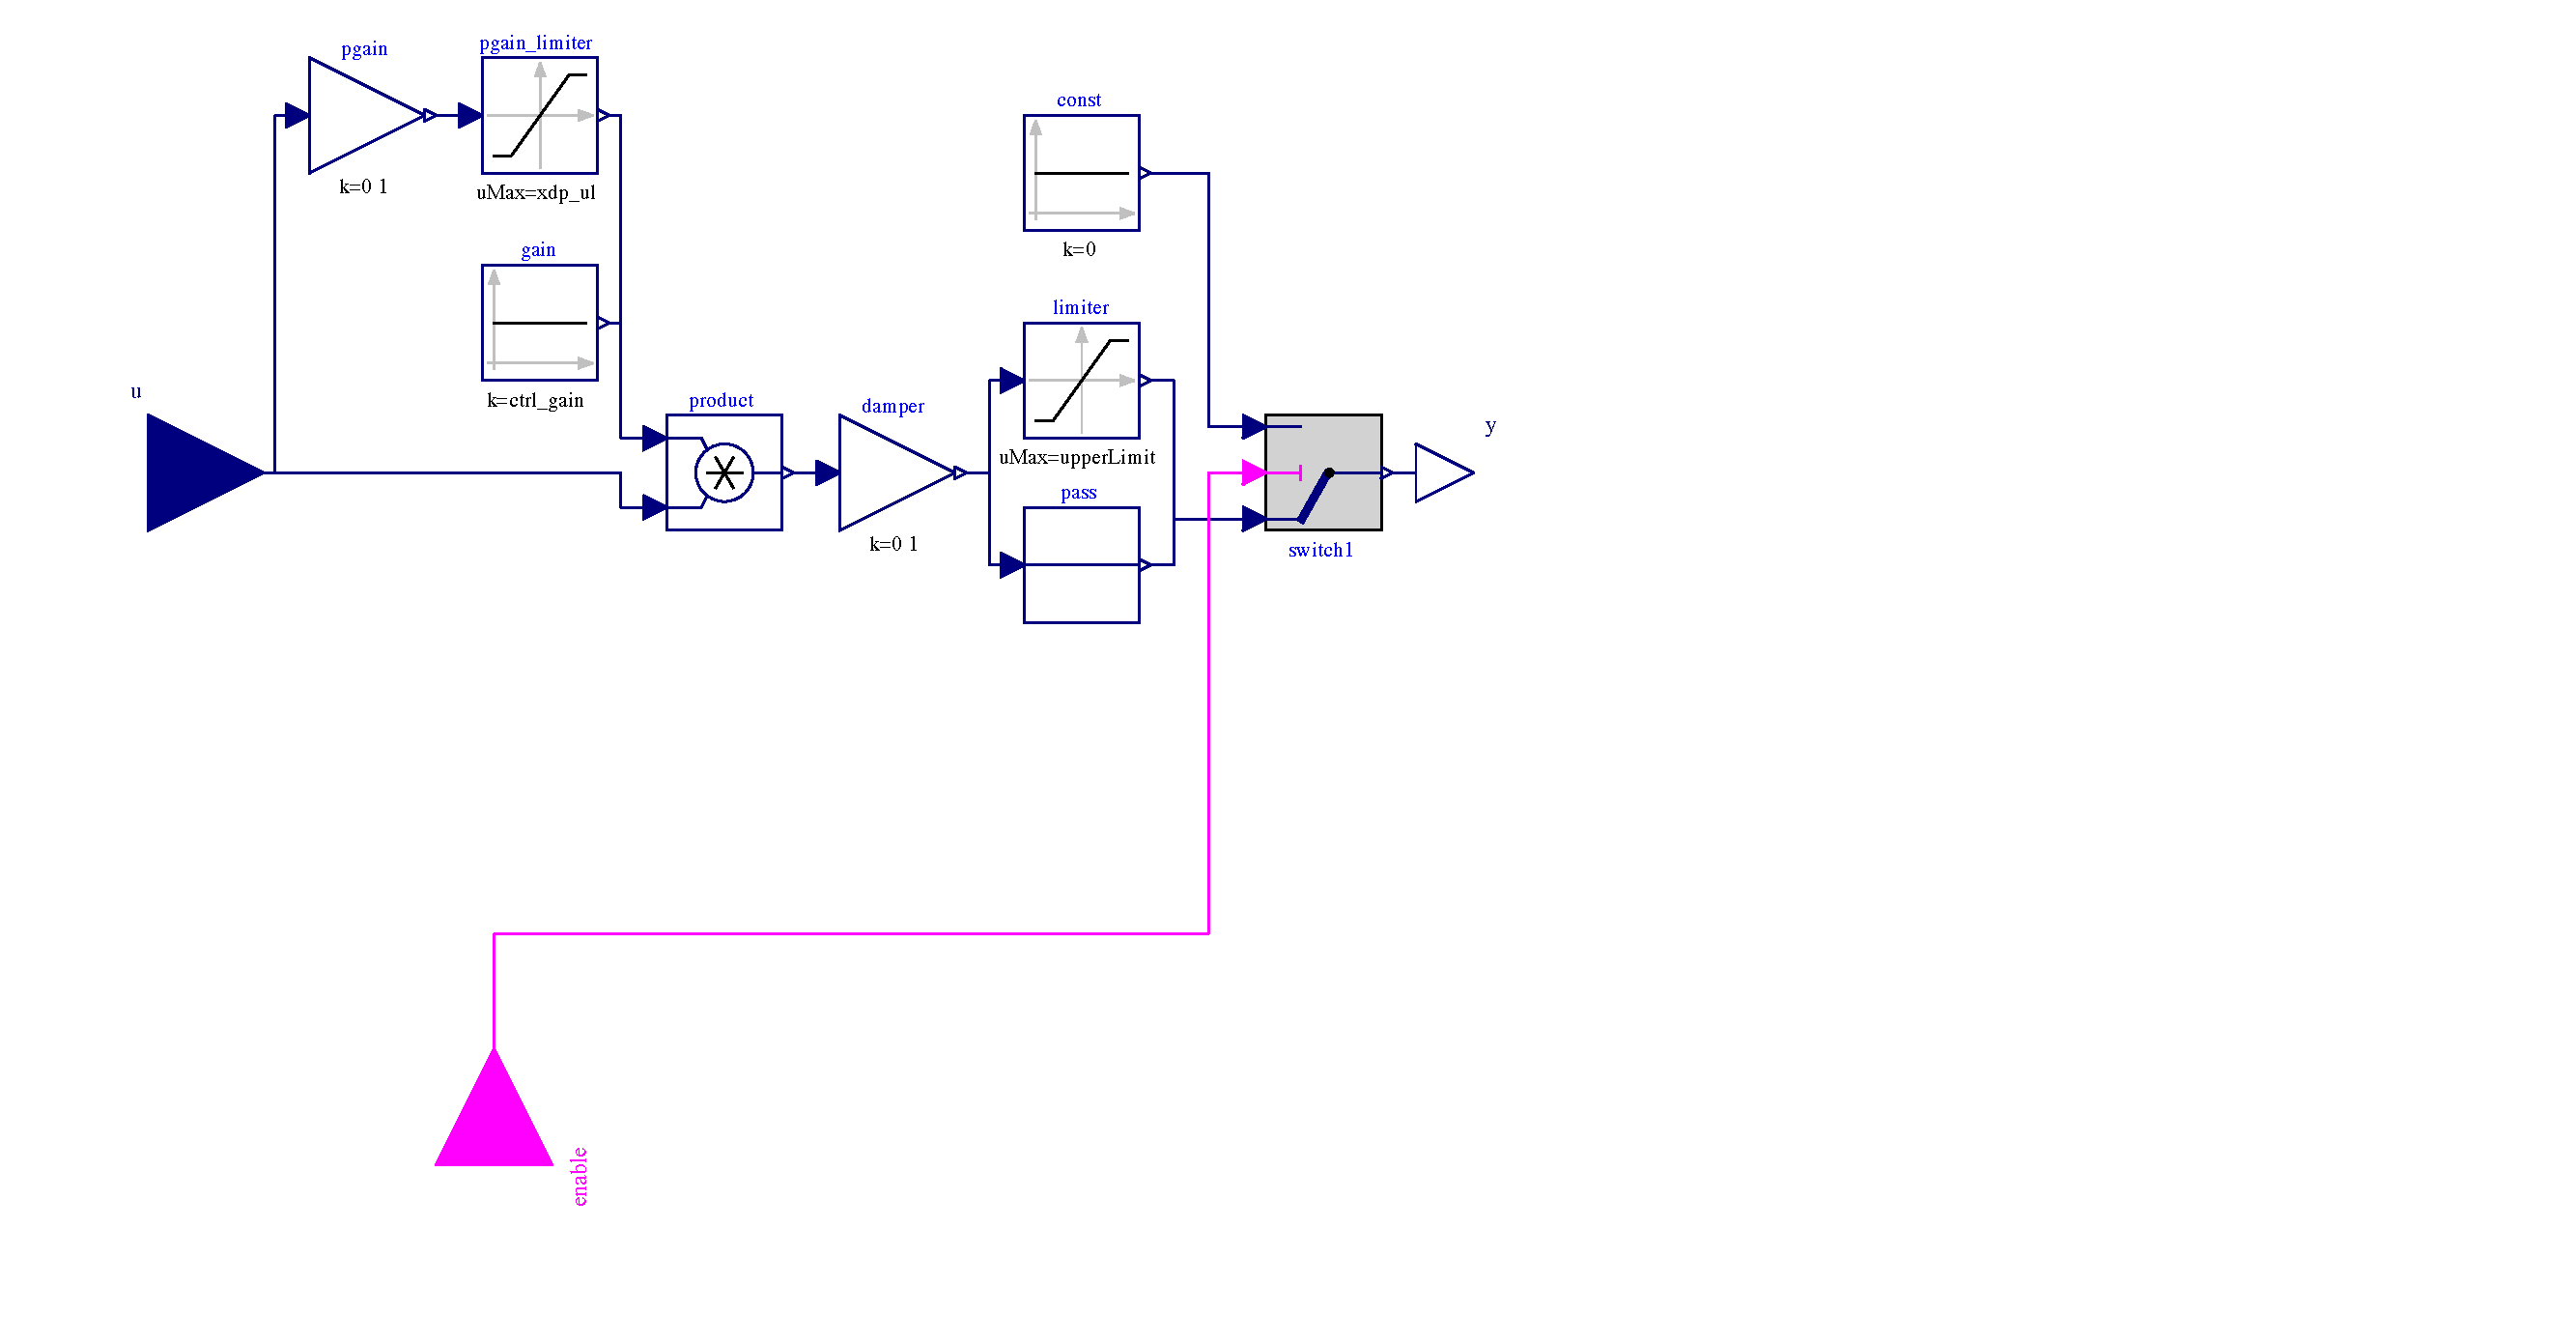
\includegraphics{Bilder/PRegler.pdf}
\caption{Modell des Proportional-Reglers
(\texttt{Frequenzumformer.Regler.Kontinuierlich.PRegler})}
\end{figure}

\begin{figure}
\centering
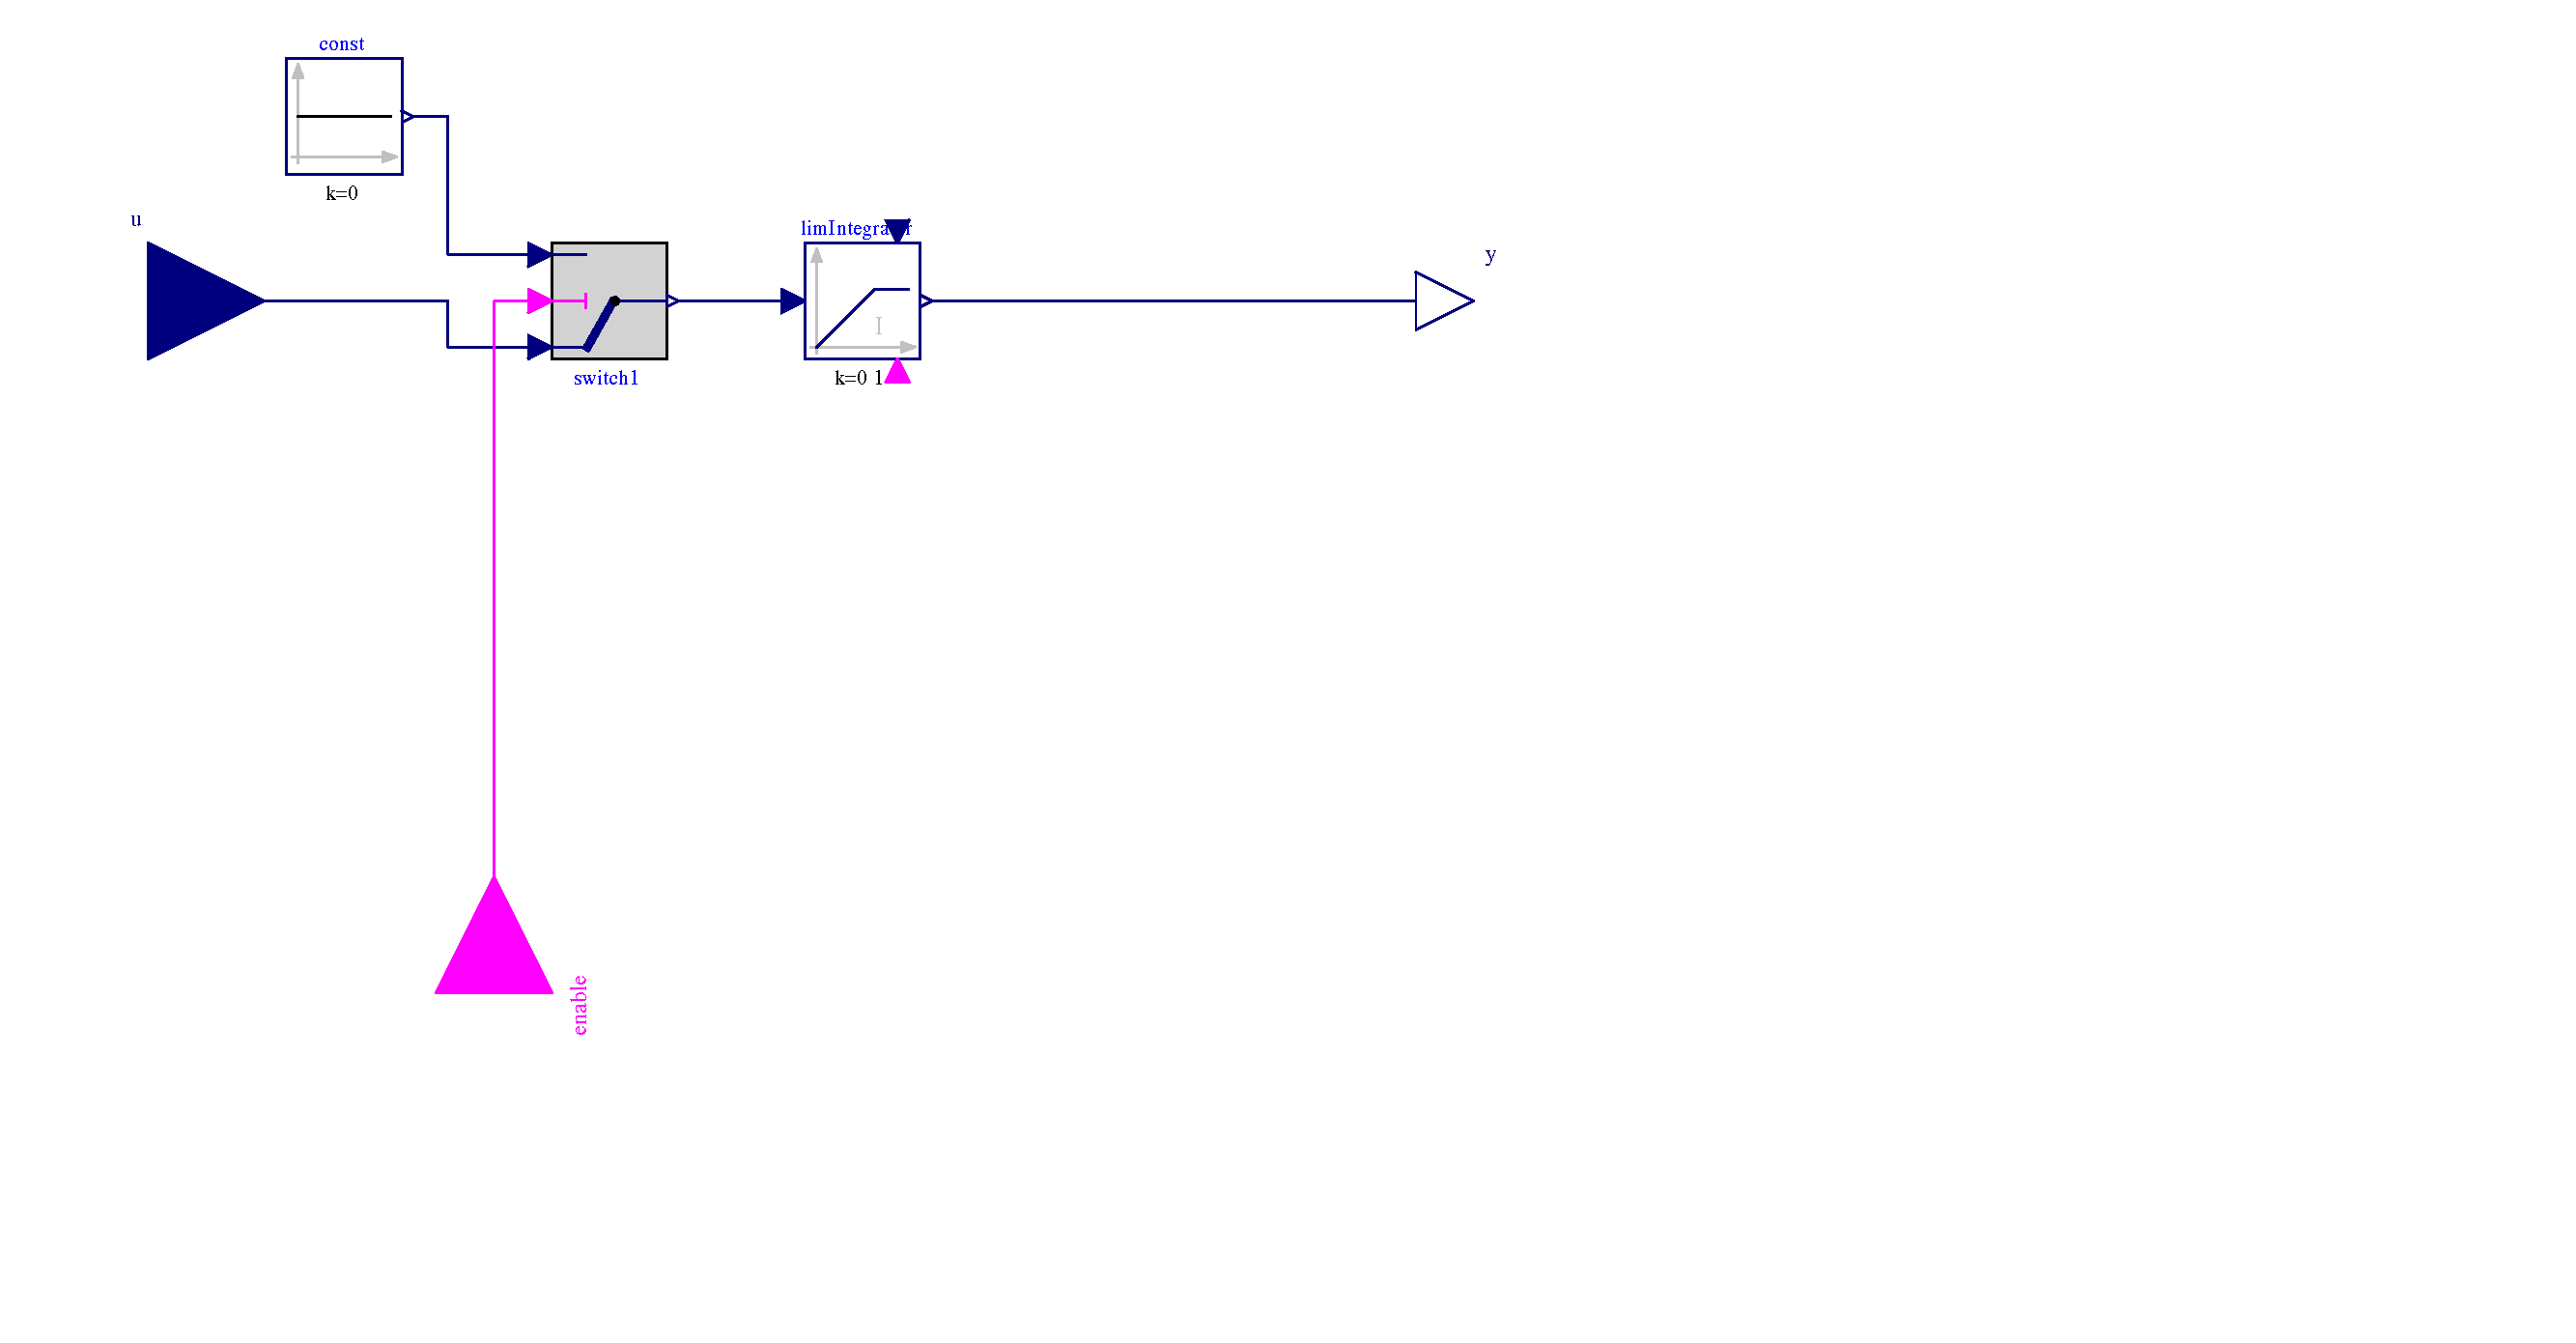
\includegraphics{Bilder/IRegler.pdf}
\caption{Modell des I-Reglers
(\texttt{Frequenzumformer.Regler.Kontinuierlich.IRegler})}
\end{figure}

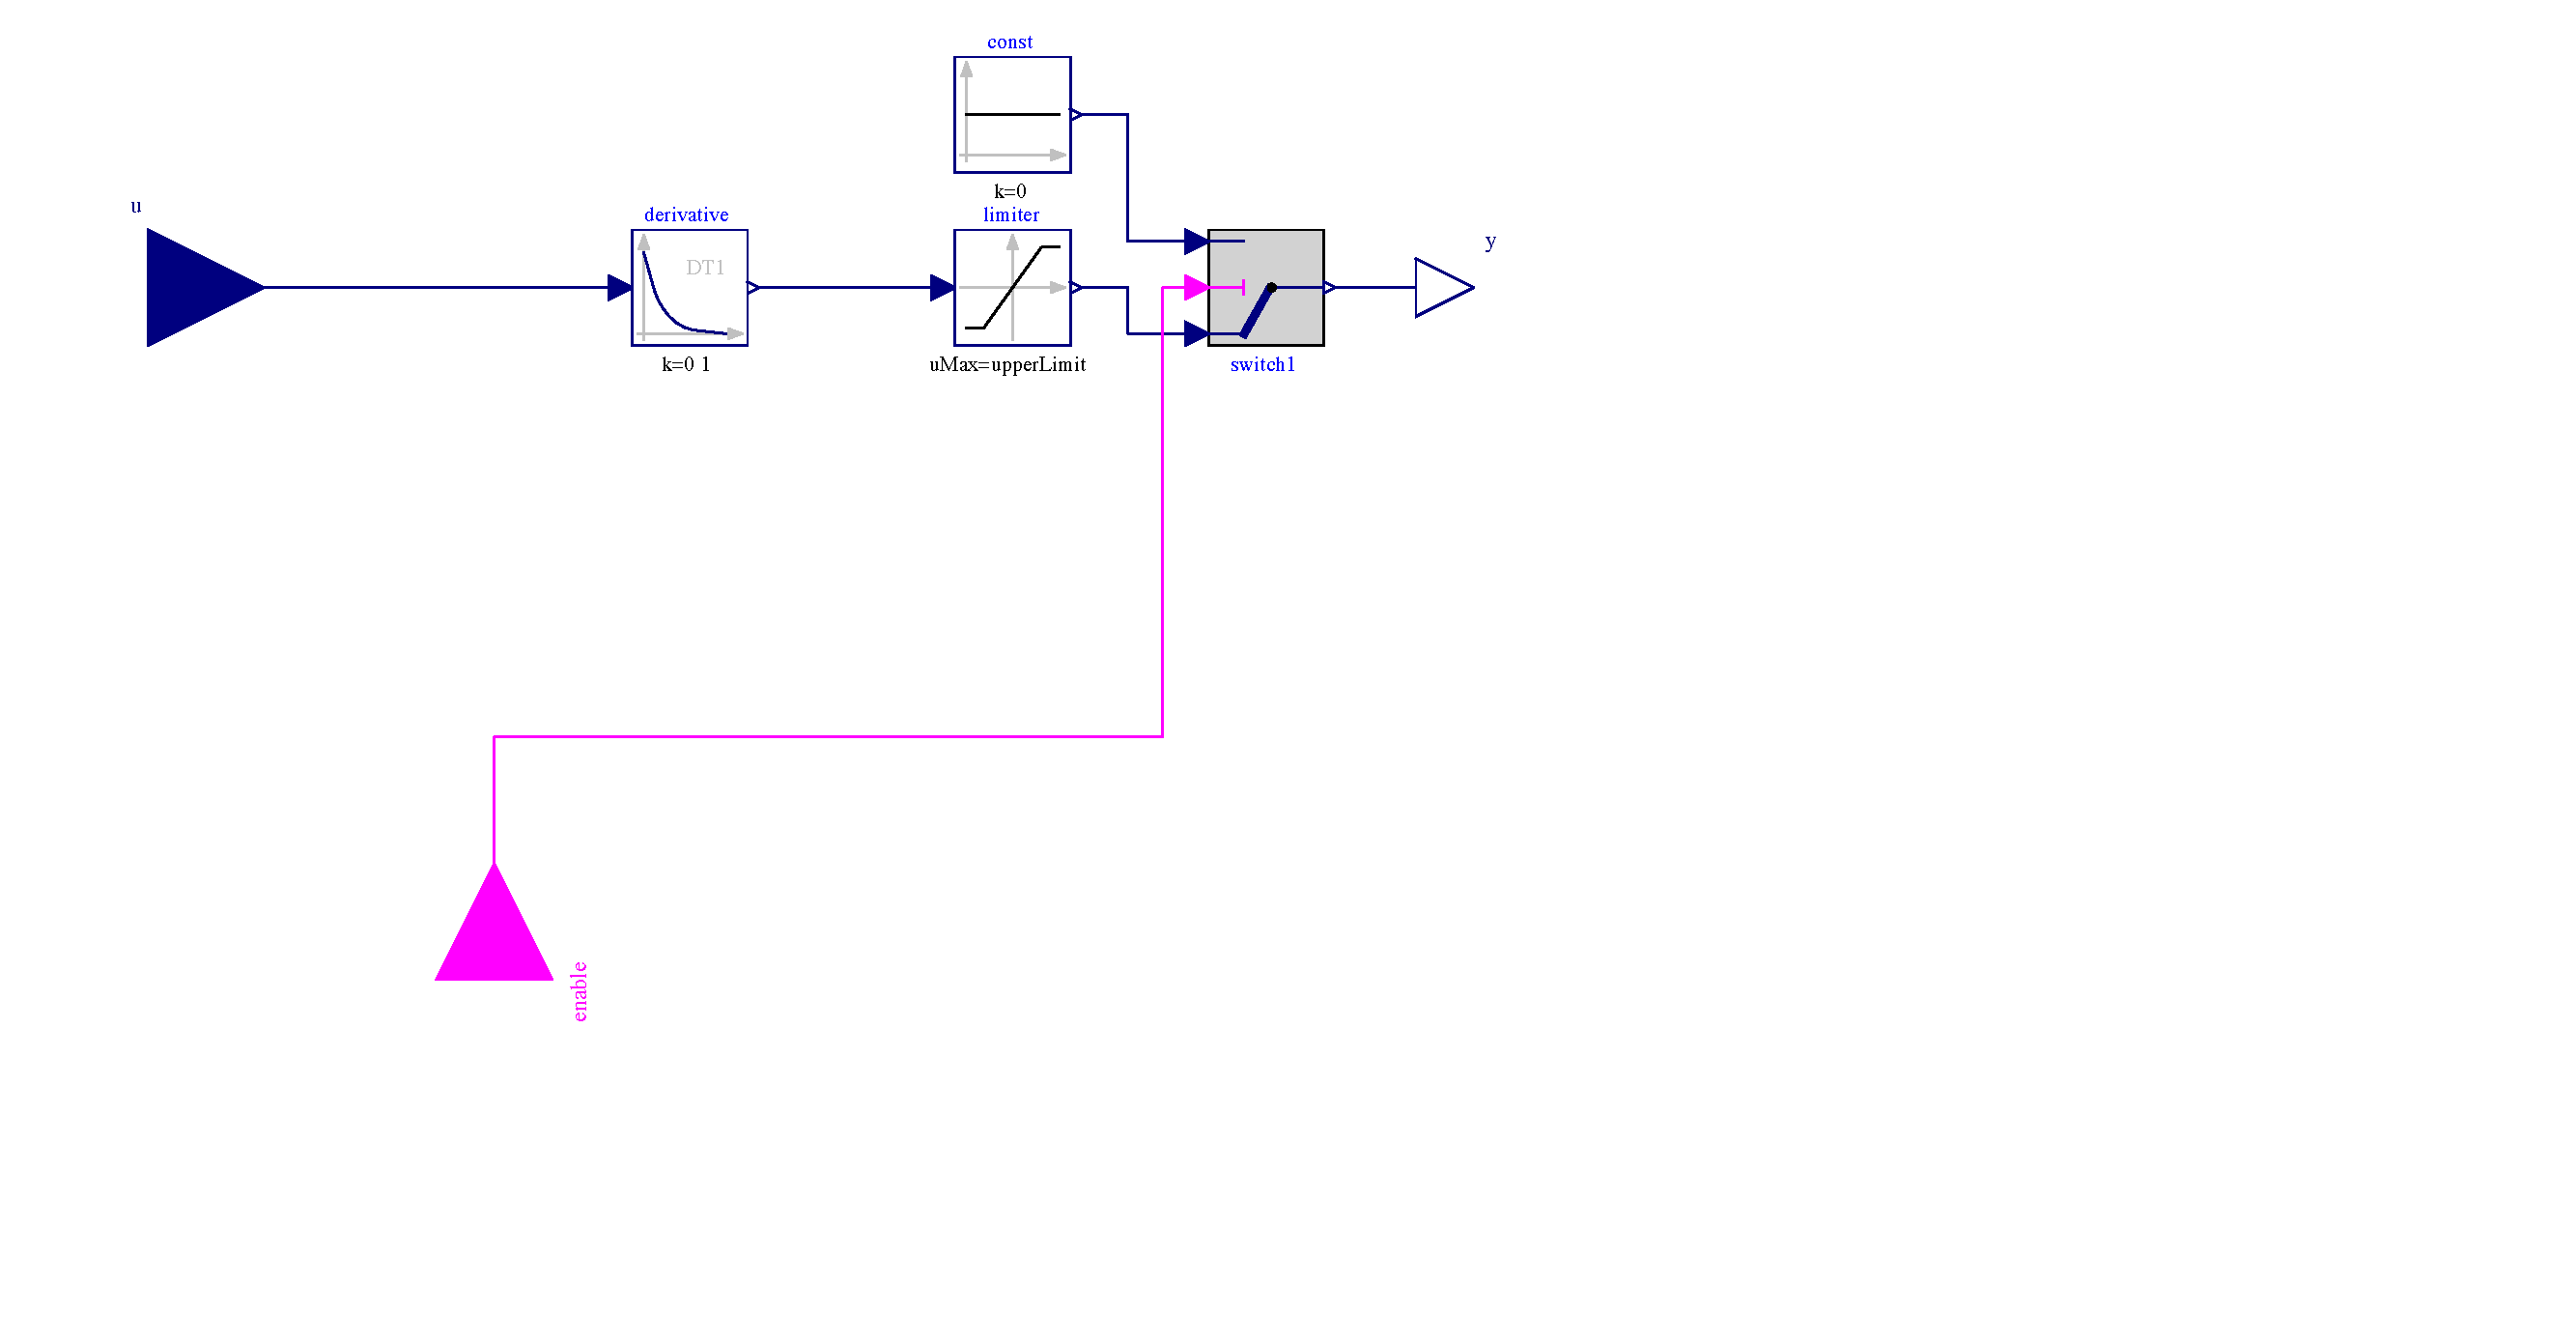
\includegraphics{Bilder/DRegler.pdf} \#\#\#\# Parametrierung

\hypertarget{umwandlungen-fuxfcr-die-reglerinternen-gruxf6uxdfen}{%
\subsection{Umwandlungen für die Reglerinternen
Größen}\label{umwandlungen-fuxfcr-die-reglerinternen-gruxf6uxdfen}}

\hypertarget{weitere-modelle}{%
\subsection{Weitere Modelle}\label{weitere-modelle}}

\hypertarget{leistungsmessung}{%
\subsubsection{Leistungsmessung}\label{leistungsmessung}}

\hypertarget{parametrierung-der-last}{%
\subsubsection{Parametrierung der Last}\label{parametrierung-der-last}}

\hypertarget{gesamtmodell}{%
\subsection{Gesamtmodell}\label{gesamtmodell}}

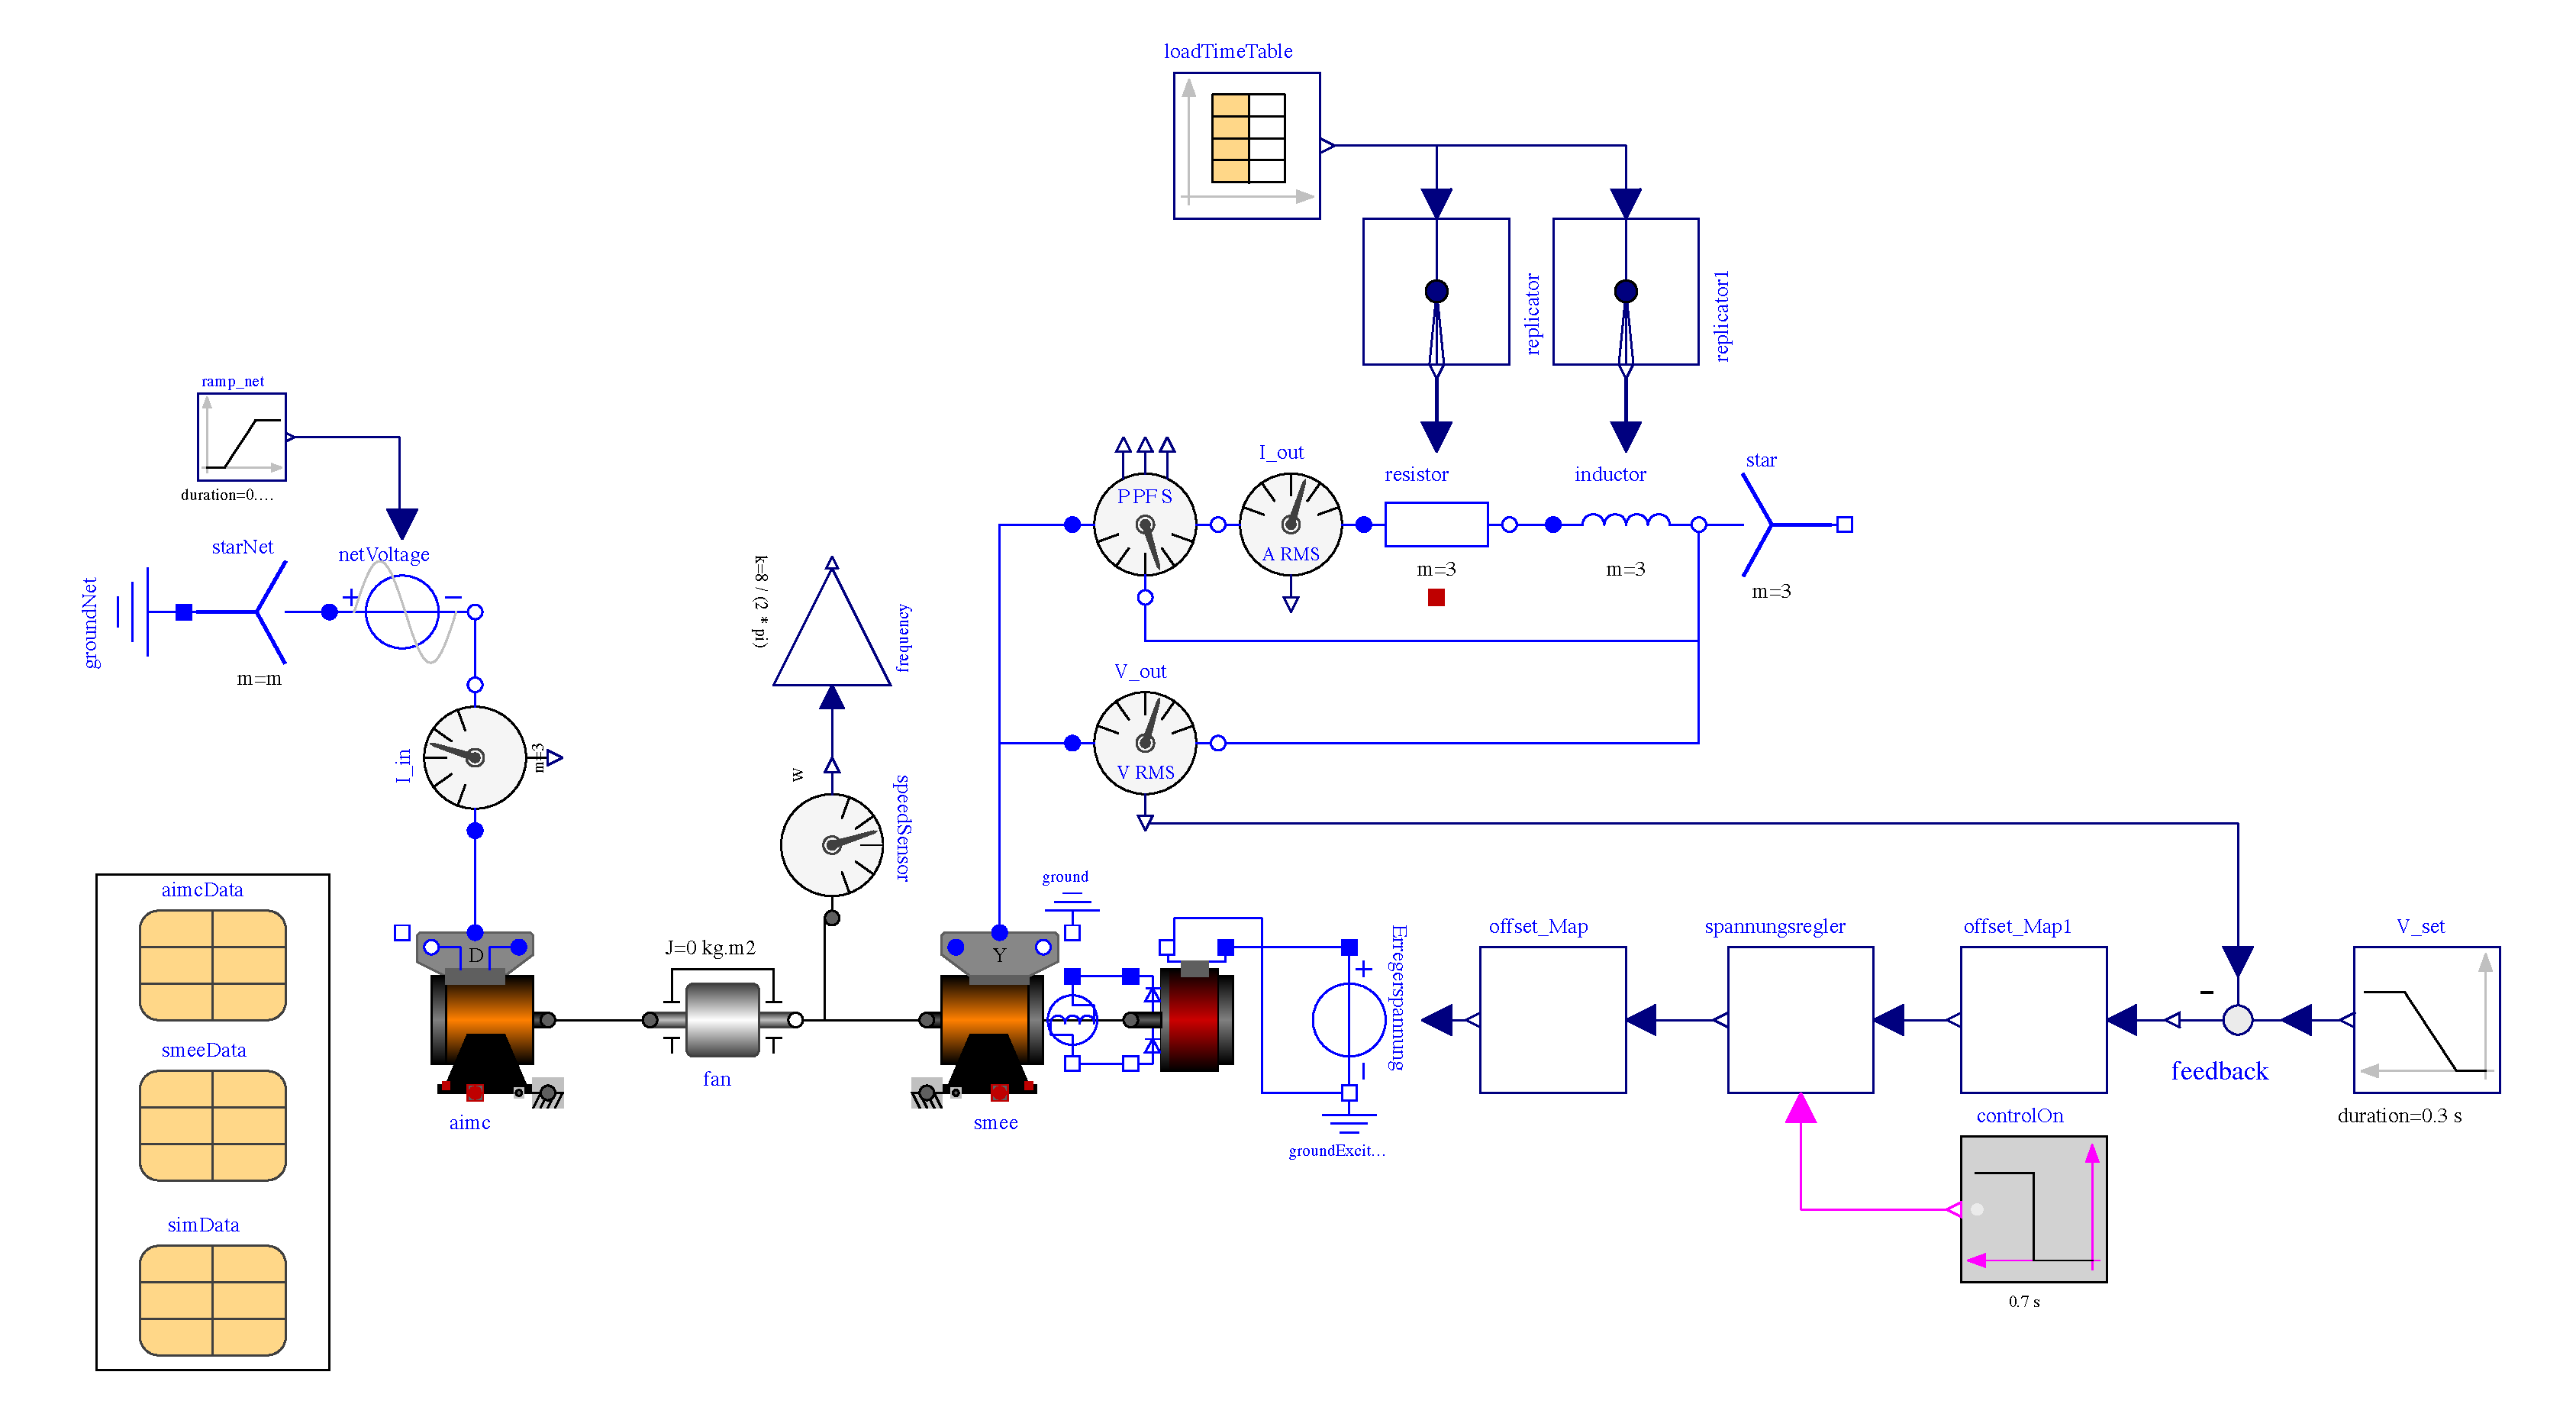
\includegraphics{Bilder/Umformer.pdf}

\hypertarget{initialisieren-des-modells}{%
\subsection{Initialisieren des
Modells}\label{initialisieren-des-modells}}

\hypertarget{muxf6gliche-quellen}{%
\section{Mögliche Quellen:}\label{muxf6gliche-quellen}}

{[}@modelicaassociationModelicaStandardLibrary2020{]}
{[}@kralModelicaObjektorientierteModellbildung2019{]}
{[}@hanseEinflussNutgeometrieAuf2020{]}
{[}@binderVorlesungElektrischeMaschinen2019{]}
{[}@bonfertBetriebsverhaltenSynchronmaschine1962{]}
{[}@IEEEGuideSynchronous{]}
